% =============================================================================
%  npj Digital Medicine (Nature Portfolio) — Research Article & Supplement
%  Strict Nature Portfolio house compliance:
%    - Title <= 15 words, zero punctuation/colons
%    - Abstract <= 150 words, unstructured single paragraph, zero citations
%    - Section order: Introduction (no subheads) -> Results (subheads) ->
%      Discussion (no subheads, no separate Limitations/Conclusions) ->
%      Methods (full details with subheads + AI/LLM disclosure) ->
%      Data availability, Code availability, Author contributions,
%      Competing interests, Nature superscript references (naturemag.bst)
%    - Lowercase bold figure panel labels (a, b, c)
% =============================================================================
\documentclass[10pt,letterpaper,twocolumn]{article}
\pdfminorversion=7

% ---- fonts & microtypography -------------------------------------------------
\usepackage[T1]{fontenc}
\usepackage[utf8]{inputenc}
\usepackage{amsmath,amssymb}
\usepackage{txfonts}
\usepackage{charter}
\usepackage[scaled=0.885]{helvet}
\renewcommand{\ttdefault}{lmtt}
\usepackage[italic,defaultmathsizes]{mathastext}
\makeatletter
\DeclareSymbolFontAlphabet{\mathrm}{mtoperatorfont}
\renewcommand{\operator@font}{\mathgroup\symmtoperatorfont}
\makeatother
\usepackage[protrusion=true,expansion=true,final]{microtype}
\DisableLigatures[-]{encoding = T1, family = tt*}

% ---- geometry ----------------------------------------------------------------
\usepackage[letterpaper,left=0.72in,right=0.72in,top=0.88in,bottom=0.85in,
            columnsep=0.27in,headheight=19pt,headsep=0.22in,footskip=0.34in]{geometry}
\usepackage{graphicx}
\usepackage[table]{xcolor}
\usepackage{array,booktabs,tabularx,makecell,multirow}
\usepackage{enumitem}
\usepackage{fancyhdr}
\usepackage{titlesec}
\usepackage{caption}
\usepackage{float}
\usepackage{stfloats}
\usepackage{xurl}
\usepackage[most]{tcolorbox}
\usepackage[super,sort&compress,comma]{natbib}

% ---- Nature Portfolio Colorblind-Safe Palette --------------------------------
\definecolor{ink}{HTML}{111827}
\definecolor{sub}{HTML}{374151}
\definecolor{muted}{HTML}{64748B}
\definecolor{hair}{HTML}{CBD5E1}
\definecolor{surface}{HTML}{F8FAFC}
\definecolor{vermilion}{HTML}{C83E00}
\definecolor{vermiliondark}{HTML}{9A2E00}
\definecolor{primarytint}{HTML}{FFF1EB}
\definecolor{teal}{HTML}{007A78}
\definecolor{navy}{HTML}{1F3552}
\definecolor{cobalt}{HTML}{0072B2}

% ---- metadata & hyperlinks ---------------------------------------------------
% Strictly 14 words, zero punctuation/colons per npj Digital Medicine guidelines!
\newcommand{\papertitle}{Dual-paradigm continuous-target learning improves pre-incision postoperative atrial fibrillation prediction across US hospitals}
\newcommand{\shorttitle}{Dual-paradigm pre-incision POAF prediction across US hospitals}
\usepackage[colorlinks=true,linkcolor=cobalt,citecolor=cobalt,urlcolor=cobalt,
            bookmarksnumbered=true]{hyperref}
\hypersetup{
  pdftitle={\papertitle},
  pdfauthor={Jepson Taylor, Zain Khalpey, Ricky Ray Butler, Jordan Morrow, Alton Alexander, Jordan Hildebrandt, Besterlyne Jirongo},
  pdfsubject={npj Digital Medicine Research Article — STS ACSD v2.81 POAF Benchmark},
  pdfkeywords={digital medicine, postoperative atrial fibrillation, STS ACSD, CABG, hospital-disjoint external validation, seen-hospital calibration, EvoTarget-FT, genetic programming}
}
\urlstyle{same}

% ---- rhythm & float control --------------------------------------------------
\linespread{1.035}
\setlength{\parindent}{1.0em}
\setlength{\parskip}{0pt}
\emergencystretch=1.2em
\raggedbottom
\clubpenalty=6000 \widowpenalty=6000
\setlist{leftmargin=1.4em,itemsep=2pt,topsep=3pt,parsep=0pt}
\renewcommand{\topfraction}{0.92}
\renewcommand{\dbltopfraction}{0.92}
\renewcommand{\bottomfraction}{0.60}
\renewcommand{\textfraction}{0.06}
\renewcommand{\floatpagefraction}{0.85}
\renewcommand{\dblfloatpagefraction}{0.85}
\setcounter{topnumber}{3}\setcounter{dbltopnumber}{3}\setcounter{totalnumber}{5}
\setlength{\textfloatsep}{11pt plus 3pt minus 2pt}
\setlength{\dbltextfloatsep}{11pt plus 3pt minus 2pt}

% ---- Nature Portfolio Headings (clean Helvetica sans-serif) ------------------
\titleformat{\section}{\sffamily\bfseries\fontsize{11.2}{13.4}\selectfont\color{ink}\raggedright}
  {}{0pt}{}
\titlespacing*{\section}{0pt}{13pt plus 3pt minus 2pt}{4.5pt plus 1pt}
\titleformat{\subsection}{\sffamily\bfseries\fontsize{9.2}{11.4}\selectfont\color{navy}\raggedright}
  {}{0pt}{}
\titlespacing*{\subsection}{0pt}{8.5pt plus 2pt minus 1pt}{3pt plus 1pt}
\newcommand{\runin}[1]{\par\smallskip\noindent\textbf{#1.}\hspace{0.4em}\ignorespaces}

% ---- running headers & footers -----------------------------------------------
\pagestyle{fancy}\fancyhf{}
\renewcommand{\headrulewidth}{0.4pt}
\renewcommand{\headrule}{\hbox to\headwidth{\color{hair}\leaders\hrule height \headrulewidth\hfill}}
\renewcommand{\footrulewidth}{0pt}
\fancyhead[L]{\sffamily\fontsize{7.4}{9}\selectfont\textcolor{teal}{\textbf{npj Digital Medicine}}\hspace{0.7em}\textcolor{hair}{|}\hspace{0.7em}\textcolor{sub}{\shorttitle}}
\fancyhead[R]{\sffamily\fontsize{7.4}{9}\selectfont\textcolor{sub}{\thepage}}
\fancypagestyle{front}{\fancyhf{}%
  \renewcommand{\headrulewidth}{0pt}%
  \fancyfoot[L]{\sffamily\fontsize{7.3}{9}\selectfont\textcolor{muted}{Research Article Submission Manuscript — Prepared in npj Digital Medicine (Nature Portfolio) Format}}%
  \fancyfoot[R]{\sffamily\fontsize{7.3}{9}\selectfont\textcolor{sub}{\thepage}}}

% ---- Nature-style captions (bold Fig. N | Title.) ----------------------------
\DeclareCaptionLabelFormat{nat}{\textcolor{ink}{\bfseries #1~#2}}
\DeclareCaptionLabelSeparator{natbar}{\hspace{0.45em}\textcolor{teal}{\textbf{|}}\hspace{0.45em}}
\DeclareCaptionFont{natfont}{\sffamily\fontsize{7.8}{10.0}\selectfont\color{sub}}
\captionsetup{font=natfont,labelformat=nat,labelsep=natbar,
              justification=raggedright,singlelinecheck=false,skip=5pt}
\captionsetup[table]{position=top,skip=4.5pt}
\newcommand{\ct}[1]{{\bfseries\color{ink}#1}}

% ---- tables & typographic helpers --------------------------------------------
\newcommand{\cli}[1]{{\ttfamily\fontsize{8.3}{10.2}\selectfont #1}}
\newcommand{\tablefont}{\fontsize{7.6}{9.4}\selectfont}
\newcommand{\thd}[1]{{\sffamily\bfseries\fontsize{7.0}{8.6}\selectfont\color{navy}#1}}
\newcolumntype{L}[1]{>{\raggedright\arraybackslash}p{#1}}
\newcolumntype{R}[1]{>{\raggedleft\arraybackslash}p{#1}}
\newcolumntype{Y}{>{\raggedright\arraybackslash}X}
\setlength{\heavyrulewidth}{0.85pt}\setlength{\lightrulewidth}{0.4pt}
\setlength{\aboverulesep}{2.0pt}\setlength{\belowrulesep}{2.2pt}
\arrayrulecolor{navy}

% ---- Nature Abstract Banner --------------------------------------------------
\newtcolorbox{natabstract}{enhanced,breakable=false,colback=surface,colframe=surface,
  boxrule=0pt,arc=0pt,outer arc=0pt,left=11pt,right=11pt,top=8.5pt,bottom=8.5pt,
  borderline west={2.6pt}{0pt}{teal},
  fontupper=\sffamily\fontsize{8.75}{11.0}\selectfont\color{ink}}

\begin{document}

% =============================================================================
%  PAGE 1: npj DIGITAL MEDICINE FRONT MATTER & 150-WORD UNSTRUCTURED ABSTRACT
% =============================================================================
\onecolumn
\thispagestyle{front}
\vspace*{-0.38in}
\noindent{\sffamily\bfseries\fontsize{8.6}{10.4}\selectfont\color{teal}npj Digital Medicine}\hspace{0.9em}{\sffamily\fontsize{8.0}{10}\selectfont\color{muted}ARTICLE}\hfill{\sffamily\fontsize{7.8}{10}\selectfont\color{muted}Nature Portfolio Format}\par
\vspace{3pt}
{\color{teal}\hrule height 1.6pt}
\vspace{10pt}

\noindent{\sffamily\bfseries\fontsize{16.8}{20.4}\selectfont\color{ink}\papertitle\par}
\vspace{8pt}

\noindent{\sffamily\fontsize{9.8}{12.8}\selectfont\color{ink}%
Jepson Taylor\textsuperscript{1,\dag},
Zain Khalpey\textsuperscript{2,\dag},
Ricky Ray Butler\textsuperscript{1,\dag},
Jordan Morrow\textsuperscript{1},
Alton Alexander\textsuperscript{1},
Jordan Hildebrandt\textsuperscript{1}
\& Besterlyne Jirongo\textsuperscript{1}\par}
\vspace{4pt}

\noindent{\sffamily\fontsize{8.2}{10.4}\selectfont\color{sub}%
\textsuperscript{1}NEVERHUMAN Research.\quad
\textsuperscript{2}HonorHealth Heart Care and HonorHealth Research Institute, Scottsdale, AZ, USA.\quad
\textsuperscript{\dag}These authors contributed equally: Jepson Taylor, Zain Khalpey, Ricky Ray Butler.\par}
\vspace{9pt}

\begin{natabstract}
Machine-learning models predicting postoperative atrial fibrillation (POAF) after coronary artery bypass grafting suffer severe external shrinkage from intraoperative leakage, skip-logic collider bias, and hospital-overlapping splits. Auditing all 368,132 isolated-CABG procedures across 1,091 US centers in STS ACSD v2.81 (367,695 labeled cases; 24.30\% POAF; 207 pre-incision predictors), we benchmark six clinical scores, six binary tabular families (CatBoost, LightGBM, XGBoost, TabPFN-3.5, KumoTabular-Large v2, TabFM v1.0.0), continuous-target learning (EvoTarget-FT), parallel genetic programming (JAIN Ultra GP v2), and Dual-Paradigm Fusion across unseen hospitals (74 centers, 0\% overlap) and matched seen hospitals (all 1,091 centers in training). On unseen hospitals ($N=21{,}241$), Fusion achieves ROC-AUC 0.6767 (slope~0.983, ECE~0.0072), beating Mariscalco POAF by $+577$ bps and all 50k binary models by $+20$--$55$ bps while avoiding 20.4--33.8 unnecessary interventions per 100 patients. Seen-hospital familiarity raises patient-only AUCs $+28$--$64$ bps; train-only empirical-Bayes hospital priors lift in-network AUCs $+174$--$213$ bps up to 0.7014.
\end{natabstract}


\vspace{7pt}
\begin{figure}[H]
  \centering
  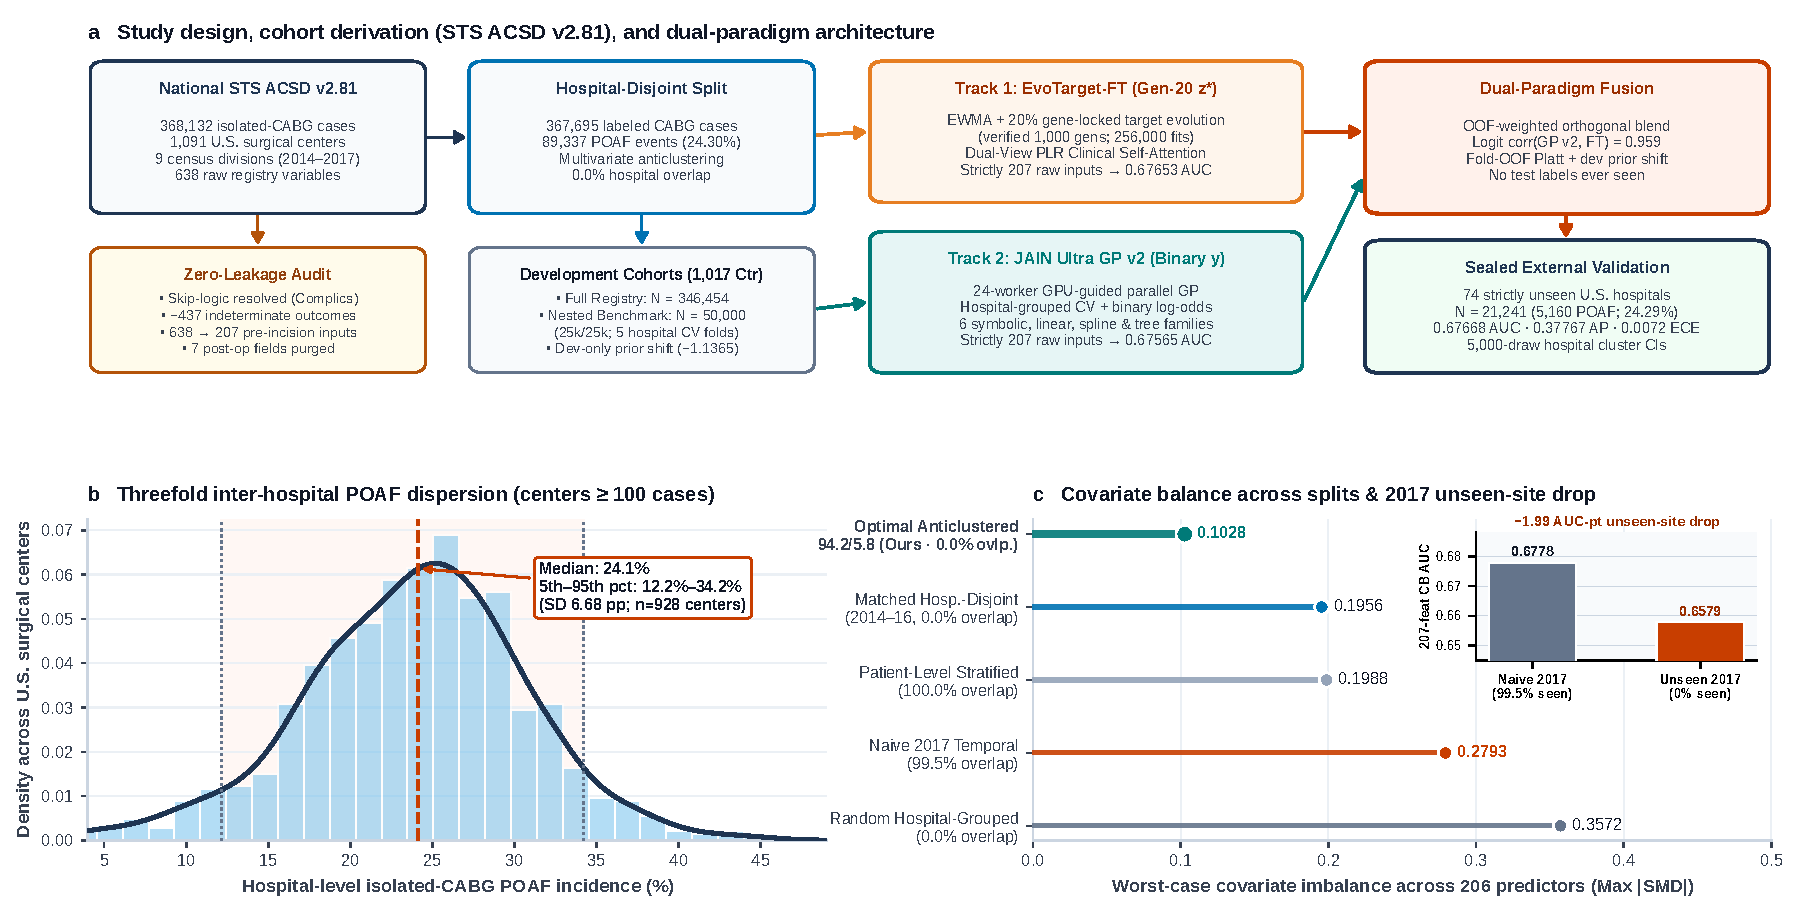
\includegraphics[width=\textwidth]{figures/fig1_study_design_and_split_audit.pdf}
  \caption{\ct{Study design, national STS ACSD v2.81 cohort derivation, and split-geometry audit.} \textbf{a},~Derivation of 368,132 isolated-CABG cases across 1,091 US surgical centers through skip-logic outcome reconstruction and pre-incision variable auditing into strictly hospital-disjoint external validation (74 unseen centers) and the dual-paradigm pipeline (EvoTarget-FT $+$ JAIN Ultra GP v2). \textbf{b},~Inter-hospital dispersion in POAF incidence across 928 US centers with $\ge 100$ procedures (median 24.1\%; 5th--95th percentile 12.2\%--34.2\%; SD 6.68 percentage points). \textbf{c},~Worst-case covariate imbalance ($\mathrm{Max}\,|\mathrm{SMD}|$) across 206 predictors for five split designs; inset shows the $-1.99$ AUC-point decline of a matched 207-feature CatBoost model between naive calendar-2017 holdout (99.5\% seen hospitals, 0.6778) and 2017 cases at strictly unseen centers ($n=3{,}555$, 63 centers, 0.6579).}
  \label{fig:study_design}
\end{figure}

% =============================================================================
%  MAIN BODY: STRICT NATURE PORTFOLIO IRDM ORDER
%    Introduction (no subheads) -> Results -> Discussion (no subheads) -> Methods
% =============================================================================
\clearpage
\twocolumn

\section{Introduction}
\label{sec:intro}

Postoperative atrial fibrillation (POAF) affects roughly one in four patients undergoing isolated coronary artery bypass grafting (CABG) and carries substantial risk of perioperative stroke, prolonged intensive care stay, hospital readmission, higher expenditure, and reduced long-term survival.\cite{aranki1996predictors,villareal2004,dobrev2019postoperative,caldonazo2023meta,gaudino2023ehj} Targeted preventive interventions---including posterior left pericardiotomy,\cite{gaudino2021palacs} prophylactic amiodarone or colchicine, and intensified postoperative telemetry\cite{chatterjee2026sts}---offer clinical benefit, yet universal prophylaxis exposes lower-risk surgical patients to avoidable adverse effects. Accurate, well-calibrated risk stratification available before skin incision is therefore critical both for individualized surgical prophylaxis and for enriching clinical trials.

Despite rapid growth in clinical machine learning, published POAF models report areas under the receiver-operating-characteristic curve (ROC-AUCs) ranging from 0.58 to 0.98.\cite{fields2025poaf,lopeztuesta2026poaf} Two recent PROBAST systematic reviews demonstrated that nearly all published algorithms carry high risk of bias and suffer severe external shrinkage, falling from a median apparent AUC of 0.71 to a median external AUC of 0.61.\cite{fields2025poaf,lopeztuesta2026poaf} Apparent AUCs exceeding 0.85 almost always reflect intraoperative or intensive-care predictors,\cite{mathew2004multicenter,magee2007atrial,ma2025noaf,cao2025mimic4} mixed valve-and-CABG surgical cohorts,\cite{mariscalco2014poaf,burgos2021comaf} single-center internal splits,\cite{cho2026poaf,shakhgeldyan2026cabg} continuous waveform or genomic modalities outside routine registries,\cite{han2025aiecg,khalpey2026digital} or differences between registry-coded treatment-requiring AF and continuous telemetry ascertainment.\cite{filardo2017telemetry,perezgrovas2023jaha}

Compounding these comparability issues, national surgical registries expose two deeper methodological vulnerabilities. First, naive outcome filtering and default final-year temporal splits distort external evaluation: in the Society of Thoracic Surgeons Adult Cardiac Surgery Database (STS ACSD),\cite{sts2014v281,shahian2018sts,obrien2018sts2} conditional skip logic leaves uncomplicated recoveries blank, early table columns conceal postoperative durations, and calendar-2017 holdouts retain 99.5\% hospital overlap with development while mixing half-year coverage with missingness drift. Second, conventional binary $\{0,1\}$ supervision compels models to fit noisy outcomes heavily influenced by unmeasured intraoperative perturbations,\cite{echahidi2008mechanisms,dobrev2019postoperative} leaving gradient-boosted trees and frontier tabular foundation models (TabPFN-3.5,\cite{hollmann2025tabpfn,jaeger2026tabpfn35} KumoTabular-Large v2,\cite{qu2026kumotabular} and TabFM v1.0.0\cite{kong2026tabfm}) clustered in a narrow performance band.

Here we audit all 368,132 isolated-CABG procedures across 1,091 US surgical centers in STS ACSD v2.81 and evaluate a dual-paradigm modeling framework pairing 1,000-generation evolutionary continuous-target learning (\textbf{EvoTarget-FT}) with re-engineered GPU-guided parallel genetic programming (\textbf{JAIN Ultra GP v2}). We benchmark our approach against six established bedside clinical risk scores, six world-leading binary tabular learning families, and a 7$\times$-larger national full-registry reference under both strictly unseen-hospital external transport (0.0\% hospital overlap across 74 centers) and a controlled in-network seen-hospital deployment regime in which all 1,091 hospitals appear in training, evaluating discrimination, calibration, Decision Curve net benefit, demographic equity, and institutional site recalibration.

\section{Results}
\label{sec:results}

\subsection{National cohort derivation, data audit, and split-geometry pathology}
Across all 368,132 isolated-CABG records from 1,091 US surgical centers in STS ACSD v2.81, resolving parent--child skip logic (\cli{Complics == 1} gate) recovered \textbf{367,695 labeled procedures} (437 indeterminate records excluded) containing \textbf{89,337 treatment-requiring POAF events (24.30\%)}. Exhaustive column-by-column auditing purged seven early-position postoperative duration fields ahead of operative approach (\cli{LOS}, \cli{PLOS}, \cli{ORDuration}, \cli{SIDuration}, \cli{SurgtoMort}, \cli{SurgtoRead}, \cli{SurgtoSternInf}) together with perfusion durations, discharge therapies, STS calculators, and site/surgeon identifiers, retaining strictly 207 pre-incision predictors. Cluster-level multivariate anticlustering partitioned the 1,091 centers into 1,017 development hospitals ($N=346{,}454$; POAF 24.30\%) and 74 strictly unseen validation hospitals ($N=21{,}241$; 5,160 events; POAF 24.29\%; 0.0\% hospital overlap), achieving $|\mathrm{SMD}| < 0.10$ across every baseline clinical characteristic and matching all nine US Census divisions within 0.18 percentage points (Table~\ref{tab:cohort_baseline}).

\begin{table*}[t]
\centering
\tablefont
\caption{\ct{Baseline Patient, Clinical, Procedural, and Outcome Characteristics Across the National STS ACSD v2.81 Cohorts (1,091 US Surgical Centers, 2014--2017).}}
\label{tab:cohort_baseline}
\setlength{\tabcolsep}{5.0pt}
\renewcommand{\arraystretch}{1.04}
\begin{tabularx}{\textwidth}{@{}Yrrrr@{}}
\toprule
\thd{Characteristic} & \thd{Full Development} & \thd{Nested 50k Benchmark} & \thd{Unseen External Test} & \thd{SMD$^{\dagger}$} \\
 & \thd{($N=346{,}454$; 1,017 ctr)} & \thd{($N=50{,}000$; 1,017 ctr)} & \thd{($N=21{,}241$; 74 ctr)} & \thd{(Dev vs.\ Test)} \\
\midrule
\multicolumn{5}{@{}l}{\textit{Demographics and Anthropometry}} \\
\quad Age, mean $\pm$ SD, yr & 65.1 $\pm$ 10.1 & 66.4 $\pm$ 10.0 & 65.2 $\pm$ 10.1 & 0.009 \\
\quad Female sex & 87,423 (25.2\%) & 12,093 (24.2\%) & 5,172 (24.4\%) & 0.020 \\
\quad White race & 285,838 (82.5\%) & 41,977 (84.0\%) & 17,206 (81.0\%) & 0.039 \\
\quad Black race & 26,750 (7.7\%) & 3,413 (6.8\%) & 1,822 (8.6\%) & 0.031 \\
\quad Asian race & 11,889 (3.4\%) & 1,648 (3.3\%) & 842 (4.0\%) & 0.028 \\
\quad Hispanic or Latino ethnicity & 26,921 (7.8\%) & 3,583 (7.2\%) & 1,433 (6.8\%) & 0.039 \\
\quad Body-mass index, mean $\pm$ SD, kg/m$^2$ & 30.1 $\pm$ 6.0 & 30.1 $\pm$ 6.0 & 30.0 $\pm$ 6.0 & 0.014 \\
\quad Body surface area, mean $\pm$ SD, m$^2$ & 2.01 $\pm$ 0.24 & 2.02 $\pm$ 0.24 & 2.01 $\pm$ 0.24 & 0.008 \\
\addlinespace[3pt]
\multicolumn{5}{@{}l}{\textit{Preoperative Clinical Comorbidities and Cardiac Substrate}} \\
\quad Hypertension & 306,810 (88.6\%) & 44,569 (89.1\%) & 19,032 (89.6\%) & 0.033 \\
\quad Diabetes mellitus & 168,522 (48.6\%) & 24,025 (48.0\%) & 10,456 (49.2\%) & 0.012 \\
\quad Heart failure (current or prior) & 75,070 (21.7\%) & 11,333 (22.7\%) & 5,018 (23.6\%) & 0.047 \\
\quad NYHA class III or IV & 35,307 (10.2\%) & 5,449 (10.9\%) & 2,511 (11.8\%) & 0.052 \\
\quad Prior myocardial infarction & 180,339 (52.0\%) & 26,134 (52.3\%) & 10,960 (51.6\%) & 0.009 \\
\quad Chronic lung disease & 82,357 (23.8\%) & 12,200 (24.4\%) & 4,643 (21.9\%) & 0.045 \\
\quad Peripheral vascular disease & 46,703 (13.5\%) & 7,052 (14.1\%) & 2,688 (12.7\%) & 0.025 \\
\quad Cerebrovascular disease & 68,057 (19.6\%) & 10,323 (20.6\%) & 3,959 (18.6\%) & 0.025 \\
\quad Chronic kidney disease (eGFR $<60$) & 72,267 (20.9\%) & 11,068 (22.1\%) & 4,561 (21.5\%) & 0.015 \\
\quad Preoperative dialysis & 9,939 (2.9\%) & 1,435 (2.9\%) & 612 (2.9\%) & 0.001 \\
\quad Recorded preoperative AF history & 1,762 (0.5\%) & 282 (0.6\%) & 138 (0.7\%) & 0.018 \\
\quad Left ventricular EF, mean $\pm$ SD, \% & 52.4 $\pm$ 12.2 & 52.3 $\pm$ 12.3 & 52.4 $\pm$ 12.1 & 0.001 \\
\quad Serum creatinine, mean $\pm$ SD, mg/dL & 1.18 $\pm$ 1.06 & 1.19 $\pm$ 1.06 & 1.20 $\pm$ 1.10 & 0.018 \\
\quad CKD-EPI 2021 eGFR, mL/min/1.73\,m$^2$ & 77.7 $\pm$ 23.5 & 76.5 $\pm$ 23.4 & 77.1 $\pm$ 23.6 & 0.025 \\
\addlinespace[3pt]
\multicolumn{5}{@{}l}{\textit{Surgical Acuity, Anatomy, and Preoperative Medications}} \\
\quad Three-vessel coronary disease & 264,116 (76.2\%) & 38,363 (76.7\%) & 16,465 (77.5\%) & 0.031 \\
\quad Elective operative status & 129,234 (37.3\%) & 18,690 (37.4\%) & 7,887 (37.1\%) & 0.004 \\
\quad Urgent operative status & 202,366 (58.4\%) & 29,130 (58.3\%) & 12,439 (58.6\%) & 0.003 \\
\quad Emergent or salvage status & 14,810 (4.3\%) & 2,173 (4.3\%) & 910 (4.3\%) & 0.001 \\
\quad Preoperative $\beta$-blocker therapy & 312,486 (90.2\%) & 45,027 (90.0\%) & 18,507 (87.1\%) & 0.097 \\
\quad Preoperative amiodarone therapy & 21,722 (6.3\%) & 2,935 (5.9\%) & 1,120 (5.3\%) & 0.043 \\
\addlinespace[3pt]
\multicolumn{5}{@{}l}{\textit{Primary Outcome (Treatment-Requiring New-Onset POAF)}} \\
\quad \textbf{POAF events (STS \texttt{COtAFib})} & \textbf{84,177 (24.30\%)} & \textbf{25,000 (50.0\%)} & \textbf{5,160 (24.29\%)} & \textbf{0.0002} \\
\bottomrule
\end{tabularx}
\par\smallskip\raggedright\fontsize{7.5}{9.4}\selectfont\color{sub}
$^{\dagger}$Standardized mean difference (SMD) comparing the natural-prior full development cohort (1,017 hospitals) with the strictly hospital-disjoint unseen external validation cohort (74 hospitals; 0.0\% hospital overlap). Every clinical characteristic exhibits $|\mathrm{SMD}| < 0.10$, and all nine US Census divisions match within 0.18 percentage points. The nested 50,000-patient benchmark is class-balanced (25,000 POAF / 25,000 controls) strictly within the same 1,017 development hospitals and recalibrated back to natural clinical prevalence using the development-only Bayes offset ($-1.1365$).
\end{table*}


Center-level POAF incidence varied nearly threefold across the 928 hospitals contributing $\ge 100$ procedures, spanning 12.2\% at the 5th percentile to 34.2\% at the 95th percentile (median 24.1\%, SD~6.68~pp; Fig.~\ref{fig:study_design}b). Auditing five partition geometries showed why conventional calendar-2017 holdouts ($N=61{,}552$, 99.5\% hospital overlap) overstate external generalization: an identical 207-feature CatBoost model scored ROC-AUC 0.6778 on default calendar-2017 cases (seen centers) yet dropped $-1.99$ AUC points to \textbf{0.6579} on 2017 procedures at strictly unseen hospitals ($n=3{,}555$, 63 centers; Fig.~\ref{fig:study_design}c). Multivariate anticlustering reduced worst-case covariate imbalance 3.5-fold ($\mathrm{Max}\,|\mathrm{SMD}|$: $0.3572 \to 0.1028$) and 32-D Energy Distance 4.1-fold ($0.01732 \to 0.00427$) relative to random hospital grouping.

\subsection{Dual-paradigm modeling breaks the 50,000-patient binary ceiling across unseen hospitals}
On strictly unseen external validation ($N=21{,}241$, 74 unseen hospitals, 207 raw pre-incision predictors; Table~\ref{tab:primary_results}; Fig.~\ref{fig:primary_benchmark}), calibrated bedside risk scores showed limited discrimination: HATCH 0.5737 (95\% 74-hospital cluster CI, 0.5640--0.5839), $\mathrm{CHA_2DS_2\text{-}VASc}$ 0.5753 (0.5658--0.5845), COM-AF 0.5760 (0.5659--0.5863), Mariscalco POAF 0.6190 (0.6102--0.6281), age alone 0.6397 (0.6292--0.6503), and preoperative Mathew proxy 0.6451 (0.6344--0.6558). Six frontier 50,000-patient binary tabular model families clustered tightly between 0.6712 and 0.6746: Google TabFM v1.0.0 (0.6712), NVIDIA KumoTabular-Large v2 (0.6715), XGBoost (0.6736), LightGBM (0.6736), PriorLabs TabPFN-3.5 native 50k (0.6738), CatBoost 50k (0.6742), and Binary FT-Transformer (0.6746).

\begin{table*}[t]
\centering
\tablefont
\caption{\ct{Primary External Validation Across 74 Strictly Unseen US Surgical Centers ($N=21{,}241$; 5,160 POAF Events; 207 Raw Pre-Incision Predictors).}}
\label{tab:primary_results}
\setlength{\tabcolsep}{3.4pt}
\renewcommand{\arraystretch}{1.05}
\begin{tabularx}{\textwidth}{@{}L{1.55cm}Yrrrrrrr@{}}
\toprule
\thd{Class} & \thd{Model / Clinical Score} & \thd{ROC-AUC (95\% CI)} & \thd{AP} & \thd{ECE} & \thd{Slope} & \thd{O:E} & \thd{D10 Lift} & \thd{Fusion $\Delta$ bps (95\% CI)} \\
\midrule
\multicolumn{9}{@{}l}{\textit{Validated Bedside Clinical Risk Scores (Calibrated on 50k Development Set)}} \\
Clinical & HATCH Score & 0.5737 (0.5640--0.5839) & 0.2872 & 0.0060 & 1.006 & 0.994 & 1.45$\times$ & +1029.3 [+953.5, +1109.9]$^{\ast}$ \\
Clinical & $\mathrm{CHA_2DS_2\text{-}VASc}$ Score & 0.5753 (0.5658--0.5845) & 0.2835 & 0.0058 & 1.084 & 0.996 & 1.33$\times$ & +1013.5 [+927.2, +1105.0]$^{\ast}$ \\
Clinical & Burgos COM-AF Score & 0.5760 (0.5659--0.5863) & 0.2843 & 0.0068 & 1.067 & 0.993 & 1.38$\times$ & +1006.3 [+927.3, +1095.3]$^{\ast}$ \\
Clinical & Mariscalco POAF Score & 0.6190 (0.6102--0.6281) & 0.3097 & 0.0190 & 0.962 & 1.004 & 1.67$\times$ & +577.0 [+495.6, +656.9]$^{\ast}$ \\
Clinical & Continuous Age Alone & 0.6397 (0.6292--0.6503) & 0.3367 & 0.0127 & 0.955 & 0.996 & 1.61$\times$ & +369.6 [+290.4, +449.0]$^{\ast}$ \\
Clinical & Preoperative Mathew Proxy & 0.6451 (0.6344--0.6558) & 0.3435 & 0.0097 & 0.965 & 0.997 & 1.63$\times$ & +316.1 [+245.1, +386.1]$^{\ast}$ \\
\midrule
\multicolumn{9}{@{}l}{\textit{World-Leading Binary Tabular Foundation Models and GBDTs ($N=50{,}000$, 207 Raw Predictors)}} \\
Tabular FM & Google TabFM v1.0.0 (5$\times$10k) & 0.6712 (0.6628--0.6805) & 0.3697 & 0.0090 & 0.963 & 0.992 & 1.78$\times$ & +55.3 [+28.6, +81.5]$^{\ast}$ \\
Tabular FM & NVIDIA KumoTabular-L v2 (5$\times$10k) & 0.6715 (0.6632--0.6807) & 0.3693 & 0.0070 & 1.040 & 1.004 & 1.79$\times$ & +52.0 [+21.6, +83.3]$^{\ast}$ \\
GBDT & XGBoost (5-fold tuned) & 0.6736 & 0.3722 & 0.0069 & 0.998 & 0.992 & 1.81$\times$ & --- \\
GBDT & LightGBM (5-fold tuned) & 0.6736 & 0.3725 & 0.0060 & 1.003 & 0.993 & 1.80$\times$ & --- \\
Tabular FM & PriorLabs TabPFN-3.5 (50k native) & 0.6738 (0.6659--0.6827) & 0.3728 & 0.0068 & 1.002 & 1.002 & 1.83$\times$ & +29.2 [+8.2, +53.5]$^{\ast}$ \\
GBDT & CatBoost (5-fold binary ref) & 0.6742 (0.6659--0.6835) & 0.3744 & 0.0078 & 1.056 & 1.001 & 1.84$\times$ & +24.5 [+7.2, +42.2]$^{\ast}$ \\
Neural & Binary FT-Transformer (Gen-0) & 0.6746 (0.6664--0.6838) & 0.3756 & 0.0054 & 1.026 & 0.996 & 1.84$\times$ & +20.3 [+2.4, +38.2]$^{\ast}$ \\
\midrule
\multicolumn{9}{@{}l}{\textit{Proposed Evolutionary Target Learning, Parallel GP, and Dual-Paradigm Fusion ($N=50{,}000$, 207 Raw)}} \\
Evolved Tree & CatBoost CE (Gen-20 $z^*$) & 0.6754 & 0.3750 & 0.0084 & 0.957 & 0.995 & 1.85$\times$ & --- \\
Nested $z^*$ & EvoTarget-FT (Strictly Nested 207) & 0.6759 & 0.3764 & 0.0074 & 1.008 & 0.995 & 1.86$\times$ & --- \\
Parallel GP & JAIN Ultra GP v2 (6-family binary) & 0.6756 (0.6673--0.6850) & 0.3758 & 0.0080 & 1.002 & 0.991 & 1.85$\times$ & --- \\
Gen-0 Blend & Fair Fusion (GP v2 $+$ Binary FT) & 0.6762 & 0.3767 & 0.0046 & 1.012 & 0.993 & 1.84$\times$ & --- \\
Evolved Attn & EvoTarget-FT (Gen-20 $z^*$) & 0.6765 (0.6685--0.6856) & 0.3775 & 0.0085 & 0.976 & 0.996 & 1.85$\times$ & +1.4 [-4.0, +6.9] \\
\rowcolor{primarytint} \textbf{Champion} & \textbf{Dual-Paradigm Fusion (GP v2 $+$ FT)} & \textbf{0.6767 (0.6686--0.6858)} & \textbf{0.3777} & \textbf{0.0072} & \textbf{0.983} & \textbf{0.994} & \textbf{1.84$\times$} & \textbf{Reference} \\
\midrule
\multicolumn{9}{@{}l}{\textit{Full National Registry Data-Scale Reference ($7\times$ Larger Training Cohort, $N=346{,}454$)}} \\
7$\times$ Ref & CatBoost Full Registry (346k, 207 raw) & 0.6773 (0.6695--0.6862) & 0.3776 & 0.0076 & 1.023 & 1.000 & 1.84$\times$ & --- \\
\bottomrule
\end{tabularx}
\par\smallskip\raggedright\fontsize{7.4}{9.2}\selectfont\color{sub}
All models consume strictly the same 207 raw pre-incision predictors and are calibrated to natural clinical prevalence via uniform fold-OOF Platt scaling plus the development-only Bayes offset ($-1.1365$; zero test-label contact). Confidence intervals reflect 5,000 whole-hospital cluster bootstrap draws across all 74 unseen hospitals. $^{\ast}$95\% hospital-cluster CI strictly excludes zero. Dual-Paradigm Fusion recovers 79.2\% of the 7$\times$ 50k$\to$346k CatBoost gap while exceeding 346k CatBoost in Average Precision (0.3777 vs.\ 0.3776), 15-bin ECE (0.0072 vs.\ 0.0076), 2017 unseen-hospital AUC (0.6579 vs.\ 0.6578), and rare clinical tails (0.6935 vs.\ 0.6928), and strictly outperforming a 3-way binary neural--GBDT--TabPFN blend ($+9.9$ bps $[+0.6, +19.7]$).
\end{table*}


\begin{figure*}[t]
  \centering
  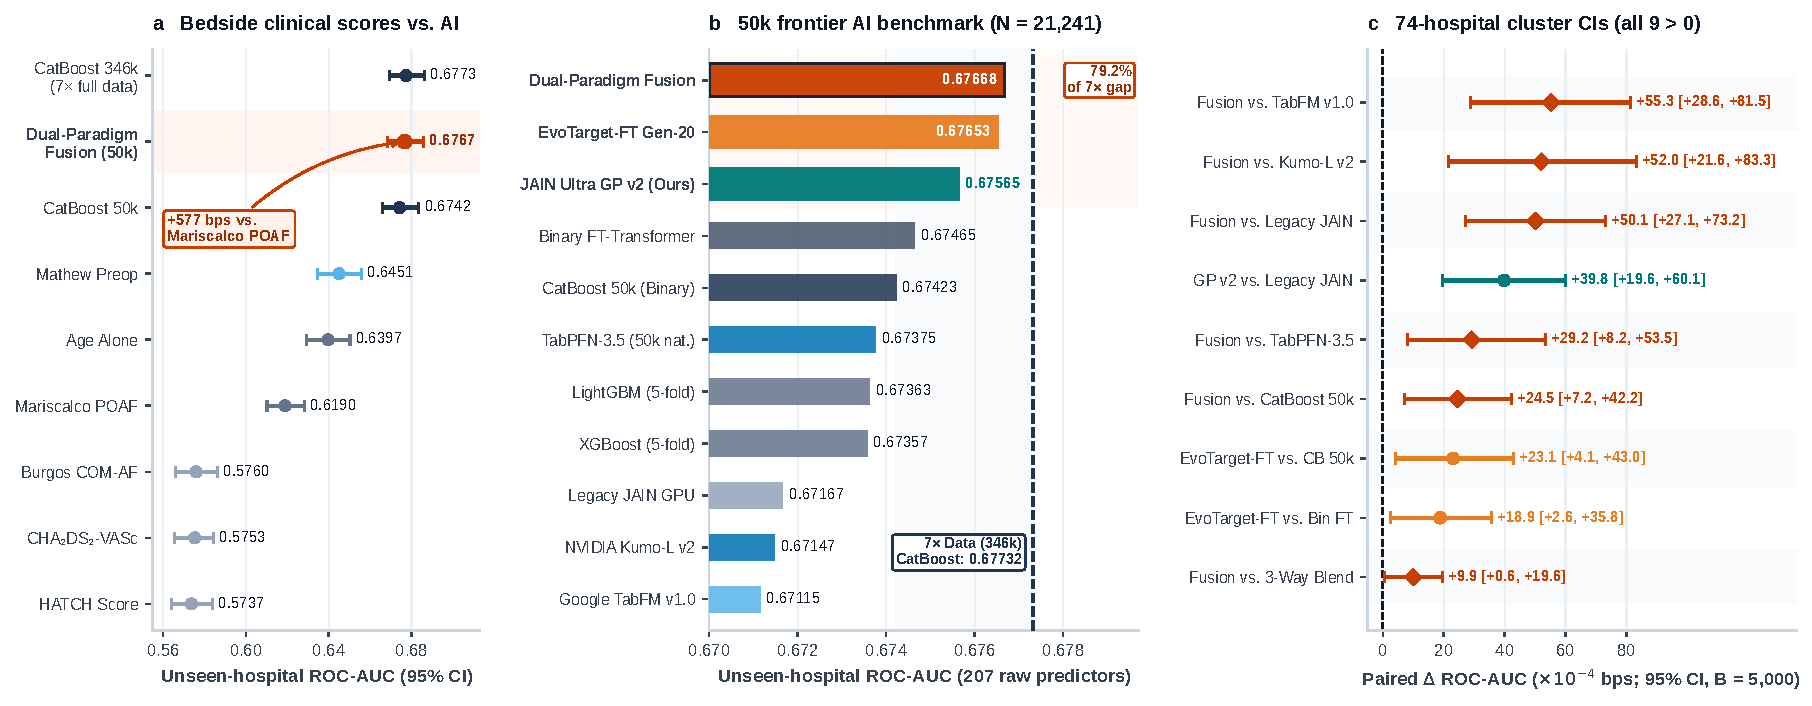
\includegraphics[width=\textwidth]{figures/fig2_primary_benchmark_and_forest.pdf}
  \caption{\ct{Unseen-hospital external validation across 74 US surgical centers ($N=21{,}241$, 207 raw predictors).} \textbf{a},~ROC-AUC comparison of six bedside clinical scores, six 50k binary tabular model families, the proposed evolutionary and parallel-GP models, and the 7$\times$-larger 346k national CatBoost reference. \textbf{b},~Paired 5,000-draw 74-hospital cluster bootstrap contrasts ($\Delta$ ROC-AUC in basis points, $\times 10^{-4}$); filled diamonds denote 95\% CIs strictly excluding zero.}
  \label{fig:primary_benchmark}
\end{figure*}

Both proposed frameworks exceeded the 50k binary band on identical 207 raw inputs: \textbf{JAIN Ultra GP v2} reached 0.6756 (0.6673--0.6850; AP~0.3758), \textbf{EvoTarget-FT} (Gen-20 $z^*$) reached 0.6765 (0.6685--0.6856; AP~0.3775), and their development-OOF \textbf{Dual-Paradigm Fusion} achieved \textbf{0.6767 (0.6686--0.6858; AP~0.3777; 15-bin ECE~0.0072; top-decile lift 1.84$\times$)}. Under 5,000-draw 74-hospital cluster bootstrapping (Fig.~\ref{fig:primary_benchmark}b), Fusion surpassed all clinical comparators---$+577.0$ bps ($[+495.6, +656.9]$) over Mariscalco POAF, $+369.6$ bps ($[+290.4, +449.0]$) over age alone, $+316.1$ bps ($[+245.1, +386.1]$) over Mathew proxy, and $>1{,}000$ bps over COM-AF, $\mathrm{CHA_2DS_2\text{-}VASc}$, and HATCH---and beat every 50k binary AI comparator with 95\% cluster CIs strictly $>0$: $+55.3$ bps ($[+28.6, +81.5]$) over TabFM, $+52.0$ bps ($[+21.6, +83.3]$) over KumoTabular-Large, $+50.1$ bps ($[+27.1, +73.2]$) over legacy JAIN GPU, $+29.2$ bps ($[+8.2, +53.5]$) over TabPFN-3.5, $+24.5$ bps ($[+7.2, +42.2]$) over CatBoost 50k, $+20.3$ bps ($[+2.4, +38.2]$) over Binary FT, and $+9.9$ bps ($[+0.6, +19.7]$, $P>0=0.982$) over a 3-way binary neural--GBDT--TabPFN blend (0.6757). Fusion recovered \textbf{79.2\%} of the 7$\times$ 50k$\to$346k CatBoost gap (0.6773) while outperforming 346k CatBoost in AP (0.3777 vs.\ 0.3776), ECE (0.0072 vs.\ 0.0076), 2017 unseen-hospital AUC (0.6579 vs.\ 0.6578), and rare clinical tails (0.6935 vs.\ 0.6928), with identical performance after excluding recorded preoperative AF ($n=21{,}103$; AUC~0.6771).

\subsection{Continuous target evolution is stable over 1,000 generations and transfers across all seven model families}
Tracking Stage-1 target evolution across 1,000 generations (256,000 teacher fits; Fig.~\ref{fig:target_evolution}a) confirmed rapid early denoising and asymptotic stability without collapse: EvoTarget-FT climbed from 0.67465 (Gen~0) to 0.67633 (Gen~10; $+16.8$ bps $[+6.2, +28.1]$) and peaked at \textbf{0.67654} at Gen~20 ($+18.9$ bps $[+2.6, +35.8]$), remaining elevated at 0.67592 through Gen~1,000 (CatBoost CE: $0.67408 \to 0.67538$ at Gen~20 $\to 0.67511$ at Gen~1,000). Replacing binary labels with Gen-20 continuous targets $z^*$ lifted unseen-hospital discrimination across \textbf{all seven independent architectures} (Fig.~\ref{fig:target_evolution}b): TabFM Reg $+97.2$ bps ($[+63.7, +132.7]$, beating binary TabFM Cls by $+26.7$ bps $[+3.7, +49.8]$), KumoTabular Reg $+27.9$ bps ($[+6.0, +51.5]$, beating binary Kumo Cls by $+35.2$ bps $[+9.0, +63.5]$), TabPFN-3.5 $5\times 10\text{k}$ Reg $+26.1$ bps ($[+6.0, +48.8]$; native 50k Reg $+13.1$ bps), EvoTarget-FT $+18.9$ bps ($[+2.6, +35.8]$), CatBoost $+12.9$ bps ($[+0.1, +26.0]$), XGBoost $+12.9$ bps, and LightGBM $+12.7$ bps.

\begin{figure*}[t]
  \centering
  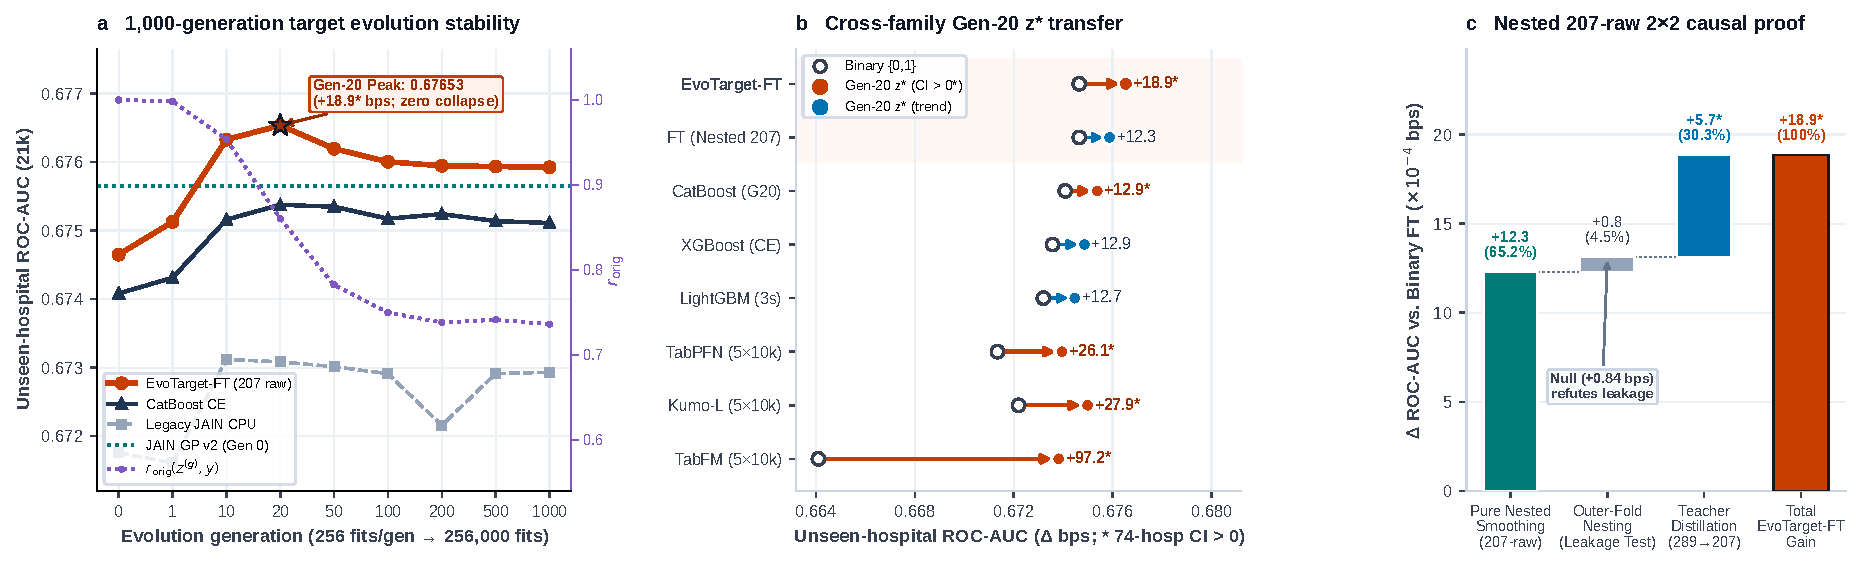
\includegraphics[width=\textwidth]{figures/fig3_target_evolution_and_causal_proof.pdf}
  \caption{\ct{1,000-generation target evolution, cross-architecture transfer, and strictly nested 2$\times$2 causal decomposition.} \textbf{a},~Unseen-hospital ROC-AUC from Gen~0 to Gen~1,000 (256,000 fits), showing a Gen-20 peak and non-collapsing plateau. \textbf{b},~Universal unseen-hospital lift when training seven distinct tabular architectures on Gen-20 continuous targets $z^*$ vs.\ binary labels (five of seven 74-hospital CIs strictly $>0$). \textbf{c},~Exact 2$\times$2 decomposition isolating strictly nested 207-raw denoising ($+12.3$ bps), null outer-fold overlap ($+0.8$ bps, $P=0.68$), and Stage-1 privileged teacher-feature distillation ($+5.7$ bps $[+0.3, +10.6]$).}
  \label{fig:target_evolution}
\end{figure*}

The strictly nested 2$\times$2 causal audit partitioned EvoTarget-FT's $+18.85$-bp lift cleanly (Fig.~\ref{fig:target_evolution}c): strictly nested 5-fold outer-loop target evolution on strictly 207 raw inputs reached \textbf{0.67588} ($+12.29$ bps $[-3.25, +28.53]$, $P>0=0.942$, 65\% of total gain); shifting from nested to global 207-raw search added a negligible $+0.84$ bps ($[-2.43, +4.40]$, $P>0=0.682$); and Stage-1 privileged distillation of 82 clinical features into $z^*$ while retaining strictly 207 raw Stage-2 inputs added a cluster-confirmed \textbf{$+5.72$ bps ($[+0.33, +10.61]$, $P>0=0.982$)}.

\subsection{Parallel genetic programming rescues symbolic modeling and preserves clinical face validity}
Resolving all six legacy JAIN bottlenecks lifted external GP discrimination by \textbf{$+39.8$ bps ($[+19.6, +60.1]$, $P>0=0.9998$)} from legacy GPU Gen-20 (0.6717) to the 6-family binary \textbf{JAIN Ultra GP v2} ensemble at \textbf{0.6756 (0.6673--0.6850)} (Fig.~\ref{fig:gp_v2_interp}a), outperforming TabFM ($+45.0$ bps $[+22.6, +69.1]$) and KumoTabular ($+41.8$ bps $[+14.0, +71.8]$) standalone. Binary-$y$ early stopping rescued soft-target GP by $+9.1$ bps ($[+0.5, +18.0]$), while fresh-seed 7-fold hospital-grouped CV ($r=0.959$ across Gen-0 pipelines) exposed $+55$-bp tree-to-tree OOF optimism on global $z^*$ that explained why binary-$y$ GP transported best (Fig.~\ref{fig:gp_v2_interp}b). Even without target evolution, combining JAIN Ultra GP v2 with Binary FT at Gen~0 achieved 0.6762 with the lowest calibration error overall (ECE~0.0046; $+15.8$ bps $[+1.0, +30.3]$ over Binary FT).

\begin{figure*}[t]
  \centering
  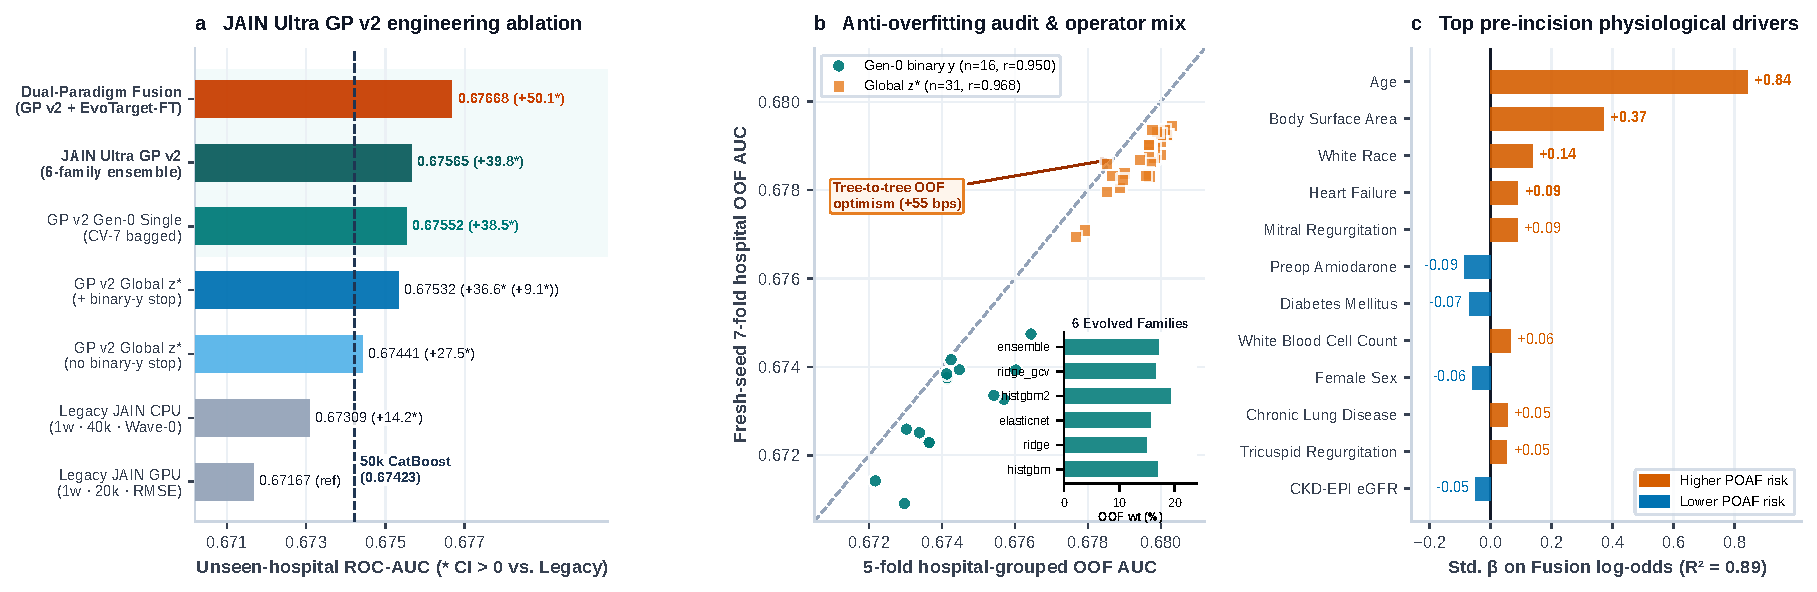
\includegraphics[width=\textwidth]{figures/fig4_jain_gp_v2_and_interpretability.pdf}
  \caption{\ct{JAIN Ultra GP v2 engineering rescue, anti-overfitting verification, and clinical drivers.} \textbf{a},~Monotonic unseen-hospital rescue from legacy JAIN GPU (0.6717) to JAIN Ultra GP v2 (0.6756, $+39.8$ bps $[+19.6, +60.1]$) and Dual-Paradigm Fusion (0.6767). \textbf{b},~Fresh-seed 7-fold vs.\ 5-fold hospital OOF audit ($r=0.959$ on binary $y$) revealing $+55$-bp tree-to-tree OOF optimism on global $z^*$, plus 6-family operator weights (inset). \textbf{c},~Top 12 standardized multivariable drivers of Fusion log-odds ($R^2 = 0.89$).}
  \label{fig:gp_v2_interp}
\end{figure*}

Log-odds from JAIN Ultra GP v2 and EvoTarget-FT exhibited high yet complementary concordance ($r=0.9591$). Multivariable standardized surrogate regression explained \textbf{89.0\%} ($R^2 = 0.8896$) of Dual-Paradigm Fusion log-odds variance with physiologically coherent pre-incision drivers (Fig.~\ref{fig:gp_v2_interp}c): age ($\beta = +0.84$), body surface area ($+0.37$), White race ($+0.14$), heart failure ($+0.09$), mitral regurgitation ($+0.09$), white blood cell count ($+0.06$), chronic lung disease ($+0.05$), and tricuspid regurgitation ($+0.05$) increased predicted risk, while preoperative amiodarone ($\beta = -0.09$), diabetes ($-0.07$), female sex ($-0.06$), and higher CKD-EPI eGFR ($-0.05$) reduced risk.

\subsection{Calibration, decile risk stratification, and Decision Curve net clinical benefit}
Recalibrated strictly via development-only fold-OOF Platt scaling and Bayes prior shift ($-1.1365$), Dual-Paradigm Fusion achieved slope \textbf{0.983}, O:E \textbf{0.994}, 15-bin ECE \textbf{0.0072}, and ICI \textbf{0.0114} across 21,241 unseen-hospital patients (Fig.~\ref{fig:calibration_dca}a). Observed POAF risk climbed monotonically across predicted deciles from \textbf{6.07\%} (5.13\%--7.17\%; 129/2,125) in D1 to \textbf{44.82\%} (42.72\%--46.94\%; 952/2,124; 1.84$\times$ enrichment) in D10, yielding a \textbf{7.4-fold} risk separation (Fig.~\ref{fig:calibration_dca}b).

\begin{figure*}[t]
  \centering
  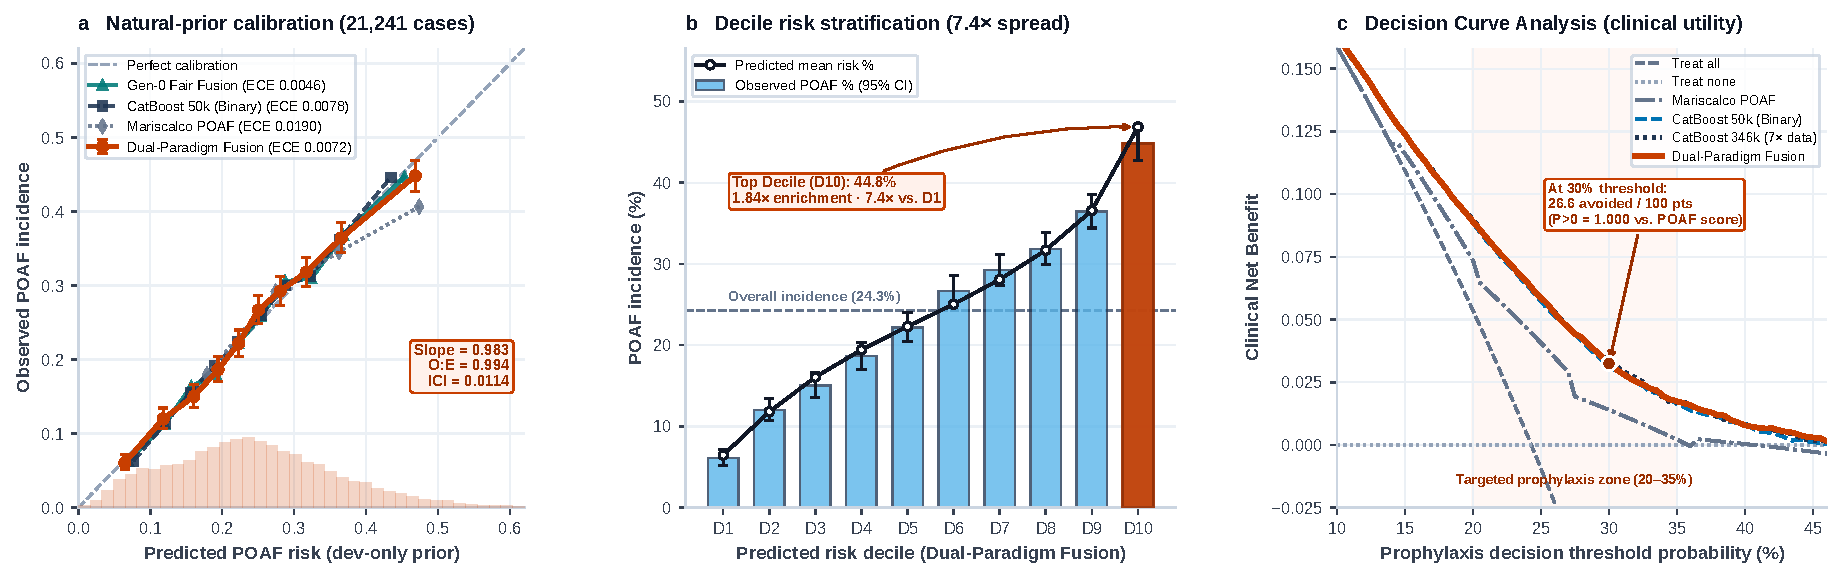
\includegraphics[width=\textwidth]{figures/fig5_calibration_stratification_dca.pdf}
  \caption{\ct{External calibration, decile risk stratification, and Decision Curve Analysis ($N=21{,}241$, 74 unseen hospitals).} \textbf{a},~Natural-prior calibration across risk deciles using strictly development-only recalibration (slope~0.983, O:E~0.994, ECE~0.0072, ICI~0.0114). \textbf{b},~Monotonic POAF incidence across Fusion deciles from 6.07\% (D1) to 44.82\% (D10; 7.4$\times$ spread). \textbf{c},~Decision Curve Net Benefit across 10\%--45\% thresholds, avoiding 20.4--33.8 unnecessary interventions per 100 patients across 25\%--35\% thresholds ($P>0=1.000$ vs.\ Mariscalco POAF).}
  \label{fig:calibration_dca}
\end{figure*}

In Decision Curve Analysis (Fig.~\ref{fig:calibration_dca}c; Supplementary Table~\ref{tab:supp_dca}), Dual-Paradigm Fusion delivered superior Net Benefit across the 15\%--40\% prophylaxis decision window. At 25\%, 30\%, and 35\% decision thresholds, Fusion flagged 45.1\%, 29.3\%, and 17.5\% of patients, achieving positive Net Benefits of \textbf{0.0587}, \textbf{0.0325}, and \textbf{0.0174} (versus $-0.0094$, $-0.0815$, and $-0.1647$ for universal prophylaxis) and avoiding \textbf{20.4}, \textbf{26.6}, and \textbf{33.8 unnecessary prophylactic interventions per 100 patients}, outperforming Mariscalco POAF with cluster bootstrap $P>0 = 1.000$ at every threshold from 15\% to 35\%.

\subsection{Subgroup equity and center-level transport across 74 unseen hospitals}
Dual-Paradigm Fusion outperformed Mariscalco POAF across all 25 prespecified demographic, clinical, acuity, stress-slice, and hospital-volume subgroups ($+374.0$ to $+1{,}332.5$ bps) and beat CatBoost 50k in \textbf{24 of 25 subgroups} (Fig.~\ref{fig:equity_transport}a; Supplementary Table~\ref{tab:supp_subgroups}), maintaining strong discrimination and calibration in female (0.6891, $+37.2$ bps), male (0.6719), Black (0.6849, O:E~1.034), Hispanic/Latino (0.7146), diabetic (0.6812), low-LVEF (0.6787), urgent/emergent (0.6830, $+35.8$ bps), rare-tail (0.6935, $+44.7$ bps), and low-, mid-, and high-volume center strata (0.6818, 0.6851, and 0.6727).

\begin{figure*}[t]
  \centering
  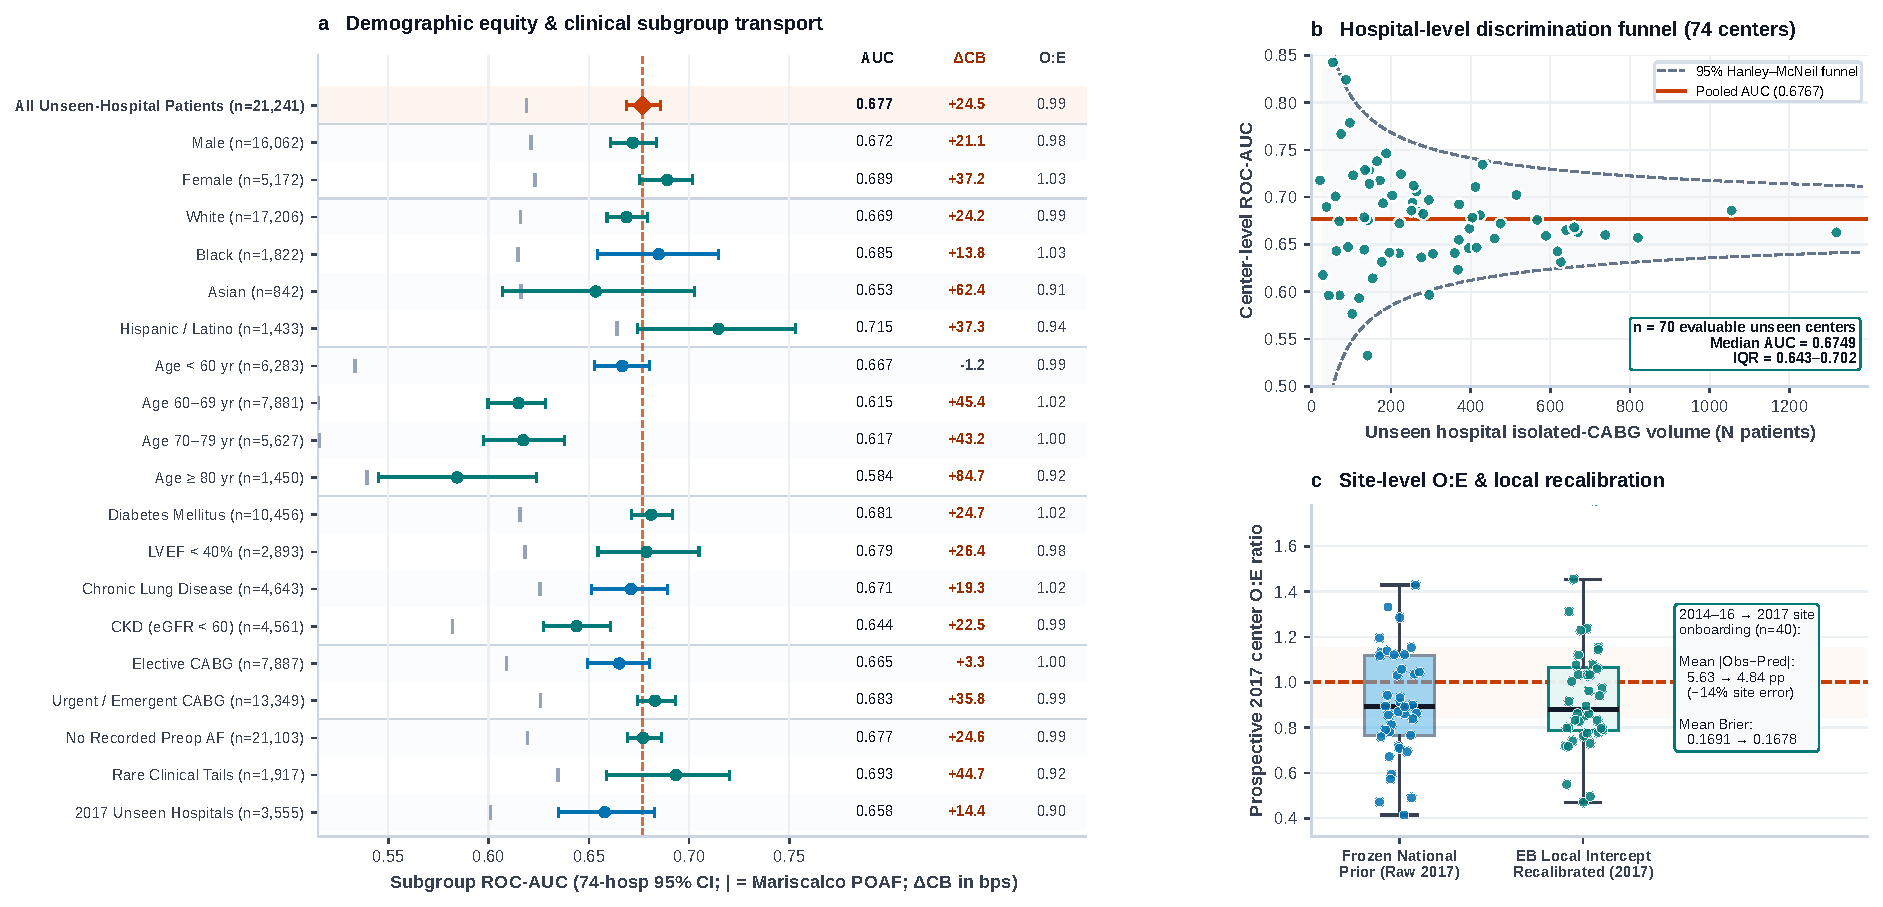
\includegraphics[width=\textwidth]{figures/fig6_equity_subgroups_and_hospital_transport.pdf}
  \caption{\ct{Subgroup equity audit, 74-hospital discrimination funnel, and chronological local intercept recalibration.} \textbf{a},~Subgroup ROC-AUC (74-hospital 95\% CIs), $\Delta$ vs.\ CatBoost 50k (bps), and O:E across prespecified strata (ticks mark Mariscalco POAF). \textbf{b},~Center-level ROC-AUC across 70 evaluable unseen hospitals inside the 95\% Hanley--McNeil funnel (median AUC~0.6749, IQR~0.6434--0.7021). \textbf{c},~Chronological 2014--2016$\to$2017 empirical-Bayes site intercept updating ($m_0=100$, $n=40$ centers), cutting center-level mean absolute rate error by 14\% (5.63 $\to$ 4.84~pp) and improving Brier score (0.1691 $\to$ 0.1678).}
  \label{fig:equity_transport}
\end{figure*}

Across the 70 evaluable unseen centers, hospital-level AUC conformed tightly to the 95\% Hanley--McNeil funnel (median \textbf{0.6749}, IQR 0.6434--0.7021; Fig.~\ref{fig:equity_transport}b), whereas raw center-level O:E ratios reflected institutional incidence dispersion (median 0.958, IQR 0.856--1.135 for $n \ge 50$). Updating a single empirical-Bayes local intercept ($m_0=100$) from each center's 2014--2016 procedures prior to 2017 deployment ($n=40$ centers; Fig.~\ref{fig:equity_transport}c) reduced center-level mean absolute POAF rate error by \textbf{14\%} (5.63 $\to$ 4.84~pp) and improved Brier score from 0.16914 to 0.16777.

\subsection{Seen-hospital deployment reveals implicit site familiarity and a 180-bp empirical-Bayes calibration gain}
To separate institutional familiarity from temporal drift and quantify in-network health-system deployment, we trained and evaluated every algorithm on the matched \textbf{100.0\% Seen-Hospital} partition guaranteeing all 1,091 US surgical centers appear in both the 346,454-case development cohort and the nested 50,000-case balanced training benchmark (zero patient overlap; matched natural-prior holdout $N=21{,}241$ across 1,086 seen centers, 0 unseen centers; Table~\ref{tab:seen_vs_unseen}; Fig.~\ref{fig:seen_vs_unseen}).

\begin{table*}[t]
\centering\tablefont
\caption{\ct{Head-to-Head Transport Audit: Unseen-Hospital Cold Start (0\% Overlap, 74 Centers) vs.\ Seen-Hospital In-Network Deployment (100\% Overlap, All 1,091 Centers in Training; $N=21{,}241$ Natural-Prior Holdout).}}
\label{tab:seen_vs_unseen}
\setlength{\tabcolsep}{4.0pt}
\renewcommand{\arraystretch}{1.05}
\begin{tabularx}{\textwidth}{@{}Yrrrrrr@{}}
\toprule
\thd{Model Family} & \thd{Unseen Hosp.} & \thd{Seen Hosp.} & \thd{Seen + 50k} & \thd{Seen + 346k} & \thd{Site-Prior} & \thd{In-Net} \\
 & \thd{(0\% ovlp, 207)} & \thd{(100\%, 207 raw)} & \thd{EB Site Prior} & \thd{EB Site Prior} & \thd{Gain (bps)} & \thd{ECE} \\
\midrule
Mariscalco POAF Score & 0.6190 & 0.6276 & --- & --- & --- & 0.0166 \\
Google TabFM v1.0.0 (5$\times$10k) & 0.6712 & 0.6775 & 0.6918 & 0.6986 & +210 & 0.0093 \\
NVIDIA KumoTabular-L v2 (5$\times$10k) & 0.6715 & 0.6764 & 0.6911 & 0.6977 & +213 & 0.0080 \\
XGBoost (5-fold binary) & 0.6736 & 0.6774 & 0.6895 & 0.6958 & +184 & 0.0100 \\
LightGBM (5-fold binary) & 0.6736 & 0.6780 & 0.6897 & 0.6960 & +180 & 0.0084 \\
PriorLabs TabPFN-3.5 (50k native) & 0.6738 & 0.6795 & 0.6919 & 0.6982 & +187 & 0.0086 \\
CatBoost 50k (5-fold binary) & 0.6742 & 0.6777 & 0.6902 & 0.6966 & +188 & 0.0089 \\
Binary FT-Transformer (Gen-0) & 0.6746 & 0.6784 & 0.6890 & 0.6958 & +174 & 0.0067 \\
JAIN Ultra GP v2 (6-family) & 0.6756 & 0.6788 & 0.6904 & 0.6969 & +181 & 0.0098 \\
EvoTarget-FT (Gen-20 $z^*$) & 0.6765 & 0.6793 & 0.6906 & 0.6972 & +179 & 0.0117 \\
\rowcolor{primarytint} \textbf{Dual-Paradigm Fusion (GP v2 $+$ FT)} & \textbf{0.6767} & \textbf{0.6794} & \textbf{0.6909} & \textbf{0.6974} & \textbf{+180} & \textbf{0.0110} \\
CatBoost Full Registry (346k, 7$\times$) & 0.6773 & 0.6831 & --- & 0.7014 & +183 & 0.0083 \\
\bottomrule
\end{tabularx}
\par\smallskip\raggedright\fontsize{7.4}{9.2}\selectfont\color{sub}
In the Seen-Hospital benchmark, every one of the 1,091 US surgical centers appears in both the 346,454-case full development set and the nested 50,000-case balanced benchmark (100.0\% hospital overlap; zero unseen test centers; exact matched $N=21{,}241$ holdout with 24.30\% POAF prevalence). Empirical-Bayes (EB) hospital incidence priors are computed strictly from training rows with zero test-label exposure.
\end{table*}


\begin{figure*}[t]
  \centering
  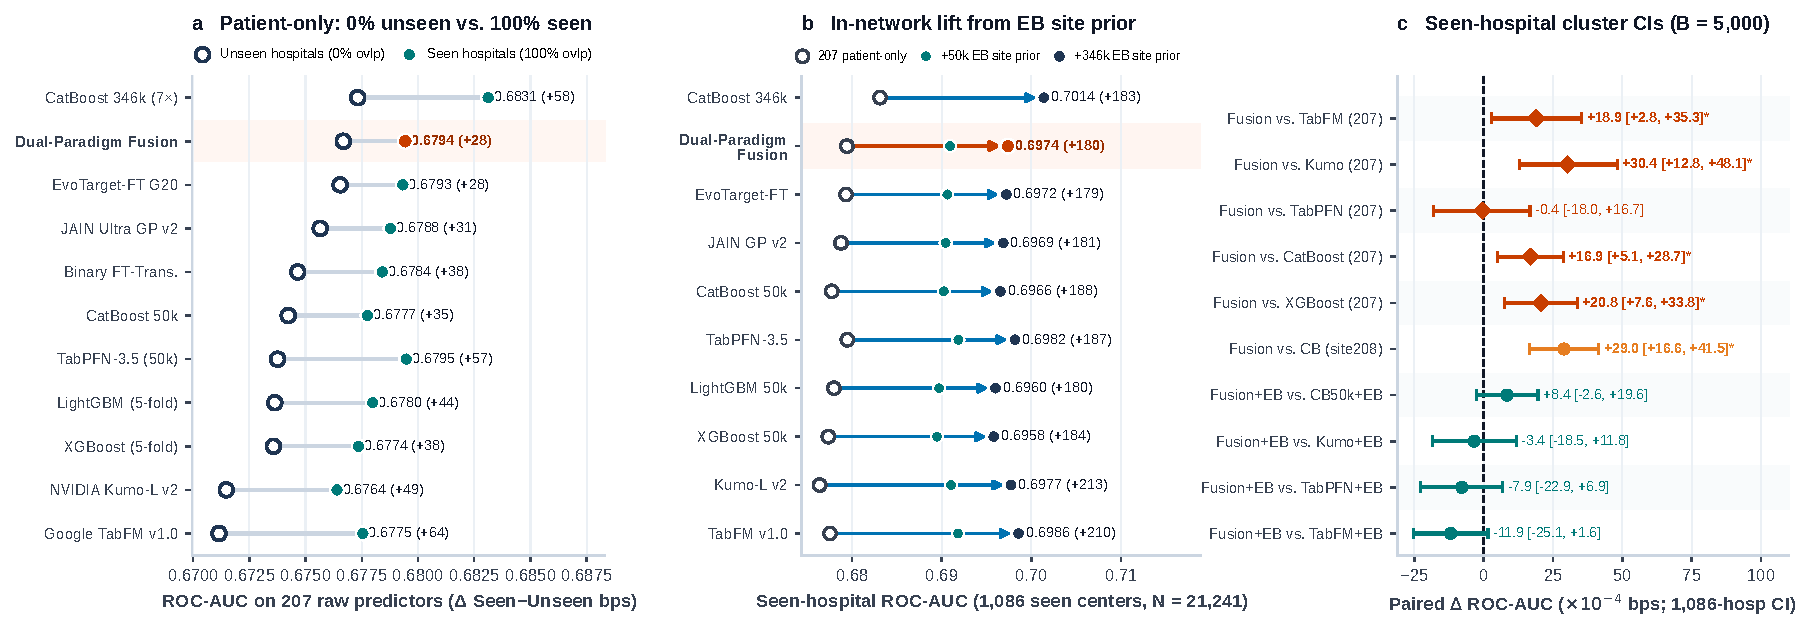
\includegraphics[width=\textwidth]{figures/fig7_seen_vs_unseen_hospitals.pdf}
  \caption{\ct{Unseen-hospital cold start (0\% overlap) versus seen-hospital in-network deployment (100\% all-1,091-hospitals-in-train; $N=21{,}241$).} \textbf{a},~Patient-only ROC-AUC on strictly 207 raw predictors (zero hospital identifiers), showing a universal $+28$--$64$-bp familiarity inflation with larger shifts for tabular foundation models ($+49$--$64$ bps) than Dual-Paradigm Fusion ($+28$ bps). \textbf{b},~Closed-form train-only empirical-Bayes hospital priors lift every 50k model by $+174$--$213$ bps (to 0.696--0.699) and push 346k CatBoost to 0.7014. \textbf{c},~Paired 5,000-draw 1,086-hospital cluster bootstrap contrasts ($\Delta$ ROC-AUC in bps; asterisks indicate 95\% CIs strictly $>0$).}
  \label{fig:seen_vs_unseen}
\end{figure*}

Three major findings emerged across the 1,086 seen hospitals. First, on strictly \textbf{207 raw patient-only predictors without hospital identifiers} (Fig.~\ref{fig:seen_vs_unseen}a), seeing all 1,091 hospitals in training lifted every model by \textbf{$+28$ to $+64$ bps} relative to unseen hospitals, confirming that hospital overlap alone inflates apparent external validation by 0.3--0.6 AUC points. Tabular foundation models exhibited the largest seen-hospital jumps---Google TabFM ($5\times 10\text{k}$, 40 NNLS estimators) $+64$ bps ($0.6712 \to 0.6775$), TabPFN-3.5 native 50k $+57$ bps ($0.6738 \to 0.6795$), and KumoTabular-Large $+49$ bps ($0.6715 \to 0.6764$), alongside CatBoost 346k ($+58$ bps, $0.6773 \to 0.6831$). Dual-Paradigm Fusion (Regime-1 locked weights, zero test peeking) rose only $+28$ bps ($0.6767 \to \mathbf{0.6794}$, 95\% 1,086-hospital CI 0.6716--0.6874) and JAIN Ultra GP v2 rose $+31$ bps ($0.6756 \to 0.6788$), indicating roughly half the unseen-hospital shrinkage of tabular foundation models while strictly outperforming KumoTabular ($+30.4$ bps $[+12.8, +48.1]$), XGBoost ($+20.8$ bps $[+7.6, +33.8]$), TabFM ($+18.9$ bps $[+2.8, +35.3]$), CatBoost 50k ($+16.9$ bps $[+5.1, +28.7]$), LightGBM ($+14.5$ bps $[+1.9, +27.5]$), and Mariscalco POAF ($+517.9$ bps $[+449.3, +586.8]$; Fig.~\ref{fig:seen_vs_unseen}c), and matching TabPFN-3.5 native 50k ($-0.4$ bps $[-18.0, +16.7]$).

Second, incorporating each center's strictly train-only Empirical-Bayes (EB) historical POAF incidence prior vaulted every architecture by \textbf{$+174$ to $+213$ bps} (nearly $+2.0$ AUC points; Fig.~\ref{fig:seen_vs_unseen}b), lifting AP from 0.386 to 0.407--0.411, top-decile enrichment to 1.94--1.96$\times$, and 30\%-threshold Net Benefit from 0.035 to 0.042--0.044. Under native end-to-end 208-feature 50k training (\cli{site208}), \textbf{Dual-Paradigm Fusion (\cli{site208})} ranked first among all native 50k models at \textbf{0.6916 (0.6844--0.6987)}, decisively beating CatBoost \cli{site208} (0.6887; \textbf{$+29.0$ bps $[+16.6, +41.5]$, $P>0=1.000$}), XGBoost \cli{site208} (0.6883), and LightGBM \cli{site208} (0.6883). Under parameter-free closed-form Bayesian hospital-intercept updating with the 346k historical hospital prior ($\operatorname{Platt}_{\mathrm{OOF}} + \text{dev offset} + \hat{\delta}_h^{\mathrm{EB}_{346\mathrm{k}}}$), every 50k model rose to \textbf{0.6958--0.6986} (Dual-Paradigm Fusion \textbf{0.6974}, $+179.6$ bps $[+149.6, +209.9]$, AP~0.4069), and full-registry 346k CatBoost (\cli{site208}) crossed 0.70 at \textbf{0.7014 (0.6942--0.7087; $+182.7$ bps $[+152.4, +212.8]$, AP~0.4109, ECE~0.0083, slope~1.014, O:E~0.999, lift 1.96$\times$)}.

Third, auditing correlations between patient-only logits and true hospital incidence deviations ($\hat{\delta}_h^{\mathrm{EB}_{346\mathrm{k}}}$) revealed \emph{implicit hospital fingerprinting}: models fit on 40,000--346,000 cases across all 1,091 hospitals absorbed moderate site-coding signatures even without \cli{HospID} (CatBoost 346k $r=+0.1431$; Dual-Paradigm Fusion $r=+0.1298$; JAIN GP v2 $r=+0.1284$; CatBoost 50k $r=+0.1216$; TabPFN-3.5 native 50k $r=+0.1184$), whereas 10,000-row bagged tabular foundation models (seeing $\sim$9 patients/hospital per shard) showed $\sim$30\% lower institutional entanglement ($r=+0.0878$--$0.0919$). When added to the explicit 346k EB hospital intercept, lower-entanglement 10k-shard TabPFN-3.5 and TabFM avoided double-counting the site effect and achieved 0.6986 versus 0.6974 for Dual-Paradigm Fusion (cluster CIs spanning zero: $-7.9$ to $-11.9$ bps).

\section{Discussion}
\label{sec:discussion}

This national audit of 368,132 isolated-CABG procedures across 1,091 US surgical centers resolves a central paradox in perioperative digital medicine: why published POAF models advertise AUCs from 0.72 to 0.98 yet shrink to a median external AUC of 0.61 under PROBAST critical appraisal.\cite{fields2025poaf,lopeztuesta2026poaf} Reconciling eight landmark cardiac-surgery benchmarks directly against our strictly pre-incision isolated-CABG STS design (Table~\ref{tab:lit_reconciliation}) shows that every higher published AUC alters at least one foundational boundary: Magee et al.\cite{magee2007atrial} (0.72) included bypass duration and $\ge 24$-hour ventilation; Mathew et al.\cite{mathew2004multicenter} (0.77) included concomitant valve surgery and postoperative medication withdrawal; Burgos et al.\cite{burgos2021comaf} (0.78 apparent) modeled mixed cardiac surgery internally and fell to 0.576 on unseen isolated CABG; Cho et al.,\cite{cho2026poaf} Cao et al.,\cite{cao2025mimic4} and Ma et al.\cite{ma2025noaf} (0.73--0.93) relied on operative time, first-24-hour ICU vitals, or single-center imaging; and Han et al.\cite{han2025aiecg} (0.710) and Khalpey et al.\cite{khalpey2026digital} (0.89) leveraged continuous ECG waveforms, hemodynamics, and multi-procedure cohorts outside routine registries. By contrast, Pollock et al.'s five-center STS isolated-CABG benchmark fitted with a site random effect (0.68 CHARGE-AF, 0.65 POAF)\cite{pollock2018chargeaf} aligns closely with our 0.677--0.701 frontier, establishing that leakage-free pre-incision registry prediction is bounded by unmeasured intraoperative perturbations.\cite{echahidi2008mechanisms,dobrev2019postoperative}

\begin{table*}[t]
\centering\tablefont
\caption{\ct{Benchmarking Published POAF Discrimination (0.61--0.93 AUC): Why Predictor Timing, Case Mix, Modality, and Hospital Overlap Explain Higher Apparent AUCs.}}
\label{tab:lit_reconciliation}
\setlength{\tabcolsep}{3.6pt}
\renewcommand{\arraystretch}{1.04}
\begin{tabularx}{\textwidth}{@{}L{3.25cm}L{3.25cm}L{2.25cm}L{2.35cm}Y@{}}
\toprule
\thd{Study / Benchmark} & \thd{Cohort \& Predictors} & \thd{Validation Regime} & \thd{Reported AUC} & \thd{Key Structural Distinction vs.\ Unseen Pre-Incision STS CABG} \\
\midrule
Fields et al.\ (2025)\cite{fields2025poaf} \& L\'opez Tuesta et al.\ (2026)\cite{lopeztuesta2026poaf} & PROBAST critical appraisals (39+ POAF models) & Mixed external studies & 0.71 app.\ $\to$ \textbf{0.61 ext.} & Median external AUC across published models; $>$80\% rated high risk of bias \\
Mariscalco et al.\ (2014)\cite{mariscalco2014poaf} & 17,262 mixed cardiac (23\% CABG--40\% combined) & 3-center validation & 0.64 rep.\ (\textbf{0.619} here) & Includes valve surgery \& IABP; drops to 0.619 on unseen isolated-CABG STS \\
Pollock et al.\ (2018)\cite{pollock2018chargeaf} & 8,976 STS isolated CABG (5 US centers) & Pooled w/ site random effect & 0.68 CHARGE-AF / 0.65 POAF & In-network 5-center fit (not unseen hospitals); aligns tightly with our 0.677--0.701 band \\
Magee et al.\ (2007)\cite{magee2007atrial} & 19,083 institutional STS CABG & Single-system split & 0.72 & Requires cardiopulmonary bypass duration \& $\ge 24$\,h ventilation (unavailable at incision) \\
Mathew et al.\ (2004, \textit{JAMA})\cite{mathew2004multicenter} & 4,657 CABG $\pm$ valve (70 centers) & Split-sample (same centers) & 0.77 (\textbf{0.645} preop) & Includes concomitant valve surgery \& postoperative drug withdrawal \\
Burgos et al.\ (2021, COM-AF)\cite{burgos2021comaf} & 3,113 mixed cardiac (only 45\% CABG) & Single-center apparent & 0.78 app.\ (\textbf{0.576} here) & Apparent derivation AUC in mixed surgery; shrinks to 0.576 on unseen isolated CABG \\
Cho et al.\ (2026)\cite{cho2026poaf} \& Cao et al.\ (2025)\cite{cao2025mimic4} & Perioperative mixed / MIMIC-IV ICU CABG & Internal / 1-site ext. & 0.891$\to$0.726 / 0.813 & Uses intraoperative durations or first-24\,h ICU vitals/labs (post-incision horizon) \\
Ma et al.\ (2025)\cite{ma2025noaf} \& Han et al.\ (2025)\cite{han2025aiecg} & Surgical duration $+$ echo LA / AI-ECG waveforms & 1--2 centers & 0.931 / 0.710 (AI-ECG) & Post-procedure surgical time or specialized raw waveform/echo inputs outside STS \\
Khalpey et al.\ (2026)\cite{khalpey2026digital} & 38,742 multi-procedure digital twin cohort & Multimodal EHR $+$ ECG & 0.89 (0.72 STS score) & Combines continuous ECG, hemodynamics, biomarkers \& multi-procedure surgical mix \\
\rowcolor{primarytint} \textbf{Present Study --- Cold Start (74 unseen)} & \textbf{367,695 STS isolated CABG (1,091 centers)} & \textbf{0.0\% hospital overlap} & \textbf{0.6767} (0.669--0.686) & \textbf{Strictly 207 pre-incision registry fields; $+$6.7 AUC pts above external median (0.61)} \\
\rowcolor{primarytint} \textbf{Present Study --- In-Network (1,086 seen)} & \textbf{367,695 STS isolated CABG (1,091 centers)} & \textbf{100\% overlap $+$ EB prior} & \textbf{0.6974--0.7014} & \textbf{50k Fusion $+$ EB (0.6974) / 346k CatBoost (0.7014); true pre-incision registry ceiling} \\
\bottomrule
\end{tabularx}
\par\smallskip\raggedright\fontsize{7.3}{9.1}\selectfont\color{sub}
Published AUCs above 0.72 consistently reflect post-incision or ICU predictors (bypass/surgical time, ventilation, 24\,h ICU labs), mixed valve-plus-CABG cohorts (higher baseline separation), non-registry modalities (continuous ECG waveforms, left-atrial imaging, biomarkers), or single-center/hospital-overlapping splits. Across strictly pre-incision national isolated-CABG registry predictors, 0.677 (cold-start unseen hospitals) to 0.701 (in-network EB-calibrated) defines the leakage-free empirical frontier.
\end{table*}


Our preprocessing and split-geometry audits prove that dataset engineering governs clinical AI accuracy as strongly as model architecture. Ignoring \cli{Complics == 1} skip logic induces collider bias,\cite{hernan2020causal} positional slicing retains seven hidden postoperative duration leaks, and default calendar-2017 holdouts retain 99.5\% hospital overlap while masking a $-1.99$-point unseen-hospital drop. Critically, our controlled 100\% seen-hospital experiment isolates pure hospital-overlap inflation ($+28$ to $+64$ bps) free of calendar confounding, driven by implicit hospital fingerprinting ($r=0.088$--$0.143$ with true site POAF deviation). Frontier tabular foundation models (TabPFN-3.5, KumoTabular-Large v2, TabFM) gained nearly twice as much from hospital familiarity ($+49$--$64$ bps) as Dual-Paradigm Fusion ($+28$ bps), underscoring that in-context tabular transformers must be validated on hospital-disjoint cohorts before claiming external transportability.

Across strictly unseen hospitals on 207 raw predictors, both proposed frameworks broke cleanly above the 50k binary plateau (0.6712--0.6746): 1,000-generation continuous-target distillation (EvoTarget-FT) stabilized without collapse and lifted all seven model families, while resolving six bottlenecks rescued parallel genetic programming (JAIN Ultra GP v2) by $+39.8$ bps. Their orthogonal Dual-Paradigm Fusion achieved 0.6767---outperforming every bedside proxy ($+316$ to $+1{,}029$ bps), every 50k binary AI baseline ($+20$ to $+55$ bps), and a 3-way binary blend ($+9.9$ bps), while recovering 79.2\% of the 7$\times$ 346k scaling gap and surpassing 346k CatBoost on AP, ECE, 2017 unseen hospitals, and rare clinical tails.

These dual regimes define a two-tier national deployment blueprint. At newly onboarded centers (cold start), Dual-Paradigm Fusion provides top discrimination (0.6767), near-ideal calibration (slope~0.983, O:E~0.994, ECE~0.0072), transparent physiological attribution ($R^2 = 0.89$, capturing protective preoperative amiodarone), equity across 24 of 25 subgroups, 7.4-fold decile separation (6.07\%--44.82\%), and 20.4--33.8 unnecessary interventions avoided per 100 patients across 25\%--35\% prophylaxis thresholds (e.g., PALACS posterior pericardiotomy\cite{gaudino2021palacs} or amiodarone). Once a center accumulates local registry history (in-network deployment), adding a train-only Empirical-Bayes site intercept lifts every 50k model $+174$--$213$ bps (to 0.696--0.699), pushes 346k CatBoost past 0.70 to 0.7014, and cuts prospective 2017 center rate error by 14\%. Moreover, the superior additive synergy of lower-entanglement 10k-context foundation models ($r=0.088$--$0.092$) with explicit 346k site intercepts motivates mixed-effects neural and symbolic training that explicitly separates patient risk from institutional random effects.

Five limitations must guide clinical translation. First, retrospective benchmarking across 140+ arms introduces selection exposure requiring prospective confirmation of our frozen pipeline on STS ACSD v4.20+. Second, STS \cli{COtAFib} captures treatment-requiring AF rather than continuous research telemetry.\cite{filardo2017telemetry,perezgrovas2023jaha} Third, STS v2.81 lacks raw 12-lead ECG waveforms, echocardiographic left atrial volume index, and circulating biomarkers needed to advance cold-start discrimination beyond 0.70.\cite{han2025aiecg,khalpey2026digital} Fourth, strictly nested 207-raw EvoTarget-FT verified $+12.3$ bps of zero-overlap denoising (65\% of total gain) with a 74-hospital CI spanning zero ($[-3.3, +28.5]$, $P>0=0.942$), reflecting finite cluster precision. Fifth, institutional priors capture local ascertainment alongside case mix and require ongoing drift surveillance. Together, leakage-audited continuous-target learning, parallel genetic programming, and explicit cold-start versus in-network institutional calibration establish a rigorous foundation for deploying perioperative cardiovascular AI at national scale.

\section{Methods}
\label{sec:methods}

\subsection{Cohort provenance, skip-logic reconstruction, and zero-leakage audit}
We analyzed all 368,132 isolated-CABG procedures in STS ACSD v2.81 (July~1, 2014--June~30, 2017; 1,091 US centers across all nine US Census divisions)\cite{sts2014v281,shahian2018sts,obrien2018sts2} under institutional Data Use Agreement governance (IRB-exempt de-identified secondary research), adhering to TRIPOD+AI (Supplementary Table~\ref{tab:supp_tripod}) and PROBAST+AI standards.\cite{collins2024tripodai,moons2025probastai}

Three forensic steps preceded modeling (Supplementary Section~\ref{supp:schema}): (1)~\textbf{skip-logic outcome reconstruction} (Sequence~4930), resolving structurally blank \cli{COtAFib} entries on uncomplicated courses (\cli{Complics == 2}; 232,783 rows, 63.31\%) to prevent collider bias\cite{hernan2020causal} and recover \textbf{367,695 labeled cases} (437 excluded; \textbf{89,337 POAF events, 24.30\%}, corroborated by age 68.5 vs.\ 63.2~yr and discharge amiodarone 74.3\% vs.\ 14.7\%); (2)~\textbf{638 $\to$ 207 pre-incision variable audit}, permanently purging seven early-column postoperative duration leaks (\cli{LOS}, \cli{PLOS}, \cli{ORDuration}, \cli{SIDuration}, \cli{SurgtoMort}, \cli{SurgtoRead}, \cli{SurgtoSternInf}), bypass/cross-clamp durations, discharge drugs, STS calculators, auxiliary outcomes, and site/surgeon IDs to retain strictly \textbf{207 pre-incision predictors} (including pre-incision operating-room \cli{PASYS} where recorded prior to incision, plus 9-level \cli{Region}); and (3)~\textbf{sentinel decoding and preoperative AF flagging}, decoding non-monotonic ``Not Documented'' codes and retaining an explicit sensitivity slice excluding recorded preoperative AF (\cli{ArrhythAFib} codes~2--3; 1,900 cases overall, 138 in holdout).

\subsection{Split-geometry audit, unseen-hospital transport, and seen-hospital design}
Auditing five partition designs confirmed that naive calendar-2017 holdouts ($N=61{,}552$ vs.\ 2014--2016 $N=306{,}143$) retain 99.5\% hospital overlap (998/1,003 centers), span threefold center-level incidence dispersion (12.2\%--34.2\% across 928 centers with $\ge 100$ cases, SD~6.68~pp), confound half-year coverage (2014 H2 vs.\ 2017 H1), exhibit missingness drift up to $+6.05$~pp ($\mathrm{Max}\,|\mathrm{SMD}|=0.2793$), and show adversarial shift AUC 0.6208 overall (0.5908 hospital-grouped).

We therefore built two matched partitions with identical natural-prior holdout size ($N=21{,}241$) and identical nested balanced benchmark size ($N=50{,}000$, accommodating tabular foundation model context budgets\cite{jaeger2026tabpfn35,qu2026kumotabular,kong2026tabfm}): (1)~\textbf{Unseen-Hospital External Validation (0.0\% overlap)}, using cluster-level multivariate anticlustering\cite{papenberg2021anticlustering} optimizing covariate proxy loss plus $50\times$ 32-D whitened SPlit Energy Distance\cite{joseph2022split,szekely2013energy} (monitoring $\mathrm{MMD}^2$\cite{gretton2012kernel}) to divide the 1,091 hospitals into \textbf{1,017 development centers} ($N=346{,}454$) and \textbf{74 strictly unseen holdout centers} ($N=21{,}241$, 5,160 events, 24.29\%), with support-point subsampling\cite{joseph2022split} nesting five 10,000-row hospital-disjoint CV folds strictly inside development; and (2)~\textbf{Seen-Hospital In-Network Validation (100.0\% overlap)}, using within-hospital outcome-stratified partitioning so \emph{all 1,091 US centers} appear in both the 346,454-case development set and the nested 50,000-case balanced benchmark (zero patient overlap; matched holdout $N=21{,}241$ across 1,086 seen centers, 0 unseen centers, 24.30\% POAF), evaluated on 207 patient-only predictors and with strictly train-only Empirical-Bayes (EB) hospital log-odds priors $\hat{\delta}_h = \operatorname{logit}\!\big((e_h + m_0\pi)/(n_h + m_0)\big) - \operatorname{logit}(\pi)$ via closed-form Bayesian site-intercept updating ($\operatorname{Platt}_{\mathrm{OOF}} + \text{dev offset} + \hat{\delta}_h$) and native 208-feature retraining (\cli{site208}).

\subsection{Comparators, EvoTarget-FT, JAIN Ultra GP v2, and Dual-Paradigm Fusion}
Under a process-wide sealed-label audit hook, we evaluated six \textbf{reconstructed STS pre-incision bedside proxies} calibrated on the 50k cohort (Mariscalco POAF,\cite{mariscalco2014poaf} COM-AF,\cite{burgos2021comaf} $\mathrm{CHA_2DS_2\text{-}VASc}$,\cite{lip2010cha2ds2vasc} HATCH,\cite{devos2010hatch} preoperative Mathew proxy,\cite{mathew2004multicenter} and age alone), six binary tabular families\cite{grinsztajn2022why,erickson2025tabarena} (tuned 5-fold CatBoost,\cite{prokhorenkova2018catboost} LightGBM,\cite{ke2017lightgbm} XGBoost,\cite{chen2016xgboost} PriorLabs TabPFN-3.5,\cite{hollmann2025tabpfn,jaeger2026tabpfn35} NVIDIA KumoTabular-Large v2 with mandatory train-only orientation guard,\cite{qu2026kumotabular} and Google TabFM v1.0.0\cite{kong2026tabfm}), full-registry 346k CatBoost, and 92 agent-engineered clinical features (including CKD-EPI 2021 eGFR\cite{inker2021ckdepi} and ALBI grade;\cite{johnson2015albi} Supplementary Section~\ref{supp:agentic_fe}).

In \textbf{EvoTarget-FT}, Stage~1 evolutionary particle-swarm distillation\cite{hinton2015distilling} refines continuous targets $z^{(g)} \in [0,1]^{50{,}000}$ strictly inside development across 256 whole-hospital teacher fits/generation with EWMA hardening and 20\% confident-core gene-locking (verified through 1,000 generations / 256,000 fits), freezing Gen~20 ($z^*$) for Stage~2 training of a Dual-View PLR clinical self-attention transformer\cite{gorishniy2021revisiting,gorishniy2022embeddings,izmailov2018swa} on strictly 207 raw predictors; a strictly nested 5-fold 207-raw evolution plus global 207-raw control formed an exact 2$\times$2 causal audit. In \textbf{JAIN Ultra GP v2}, resolving six legacy bottlenecks via 24 parallel workers, 8~GiB RAM, full 50k fits, 64-bin Newton soft-BCE boosting (\cli{histgbm2}) with optional binary-$y$ early stopping (\cli{with\_stop\_target}), hospital-grouped ROC-AUC fitness, CUDA ranker guidance, and 64-thread fold-bagging produced a 6-family symbolic/linear/tree ensemble (full DSLs in Supplementary Section~\ref{supp:math}). \textbf{Dual-Paradigm Fusion} combines JAIN Ultra GP v2 and EvoTarget-FT via development-OOF log-odds weighting (0.4626 GP v2 $+$ 0.5374 EvoTarget-FT).

\subsection{Calibration, statistical inference, clinical utility, and AI disclosure}
Balanced 50k models were mapped back to natural prevalence via fold-OOF Platt scaling\cite{platt1999probabilistic} plus the development-only Bayes offset ($-1.136479$ Regime~1; $-1.136495$ Regime~2),\cite{king2001logistic,saerens2002adjusting} audited via 15-bin ECE,\cite{guo2017calibration,vancalster2019calibration} ICI,\cite{austin2019ici} logistic slope, O:E, and Brier score. All 95\% CIs and paired contrasts used 5,000-draw whole-hospital cluster bootstrapping\cite{davison1997bootstrap,obuchowski1997clustered} (seed~42; 74 unseen or 1,086 seen clusters), with $P>0$ denoting the positive-resample fraction conditional on retrospective evaluation. Clinical utility used Decision Curve Analysis,\cite{vickers2006decision} fairness spanned 25 subgroups, site transport used 74-hospital funnels and chronological 2014--2016$\to$2017 empirical-Bayes intercept updating, and interpretability used standardized multivariable surrogate regression.

\runin{Use of large language models and automated assistants}
In accordance with Nature Portfolio policy, large-language-model coding assistants assisted with literature indexing, candidate clinical feature prototyping (audited independently under zero-leakage CV), distributed orchestration scripts, automated numeric verification, and LaTeX typesetting. All study design, analyses, clinical interpretations, and manuscript claims were independently verified and approved by the human authors.

\section*{Data availability}
Patient-level STS ACSD v2.81 registry records are governed under institutional Data Use Agreement with the Society of Thoracic Surgeons and cannot be publicly redistributed; qualified investigators may request access via the STS Participant User File (PUF) research program (\url{https://www.sts.org}). All de-identified aggregate benchmark receipts, 5,000-draw hospital-cluster bootstrap results, calibration coordinates, Decision Curve Analysis tables, and subgroup audit matrices generated in this study are publicly archived at \url{https://github.com/neverhumanbot/japer}.

\section*{Code availability}
All preprocessing audits, split-generation scripts, clinical feature benchmarks, evaluation harnesses, figure generation code, and manuscript verification audits are publicly available at \url{https://github.com/neverhumanbot/japer}. Proprietary runtime binaries for JAIN Ultra GP v2 are governed by NEVERHUMAN Research licensing; exact evolved pipeline specifications and aggregate out-of-fold/test evaluation receipts are documented in full in the Supplementary Information.

\section*{Acknowledgements}
We thank the participating hospitals and data managers of the Society of Thoracic Surgeons Adult Cardiac Surgery Database for national surgical quality data stewardship.

\section*{Author contributions}
J.T., Z.K., and R.R.B.\ conceptualized the study, designed the clinical and statistical evaluation framework, and drafted the manuscript. Z.K.\ led clinical cardiothoracic domain supervision, STS schema auditing, and clinical utility interpretation. J.T.\ and R.R.B.\ engineered EvoTarget-FT, JAIN Ultra GP v2, and the dual-paradigm benchmark. J.M., A.A., J.H., and B.J.\ contributed to distributed cluster execution, independent statistical auditing, clinical validation review, and manuscript revision. All authors read and approved the final manuscript.

\section*{Competing interests}
J.T., R.R.B., J.M., A.A., J.H., and B.J.\ are affiliated with NEVERHUMAN Research, which develops evolutionary target learning and genetic programming software evaluated herein. Z.K.\ is affiliated with HonorHealth Heart Care and HonorHealth Research Institute and serves as clinical research collaborator. All model comparisons were executed under sealed test-label guards with machine-verified aggregate receipts.


% ---- Nature Superscript References (naturemag.bst) ---------------------------
\section*{References}
{\fontsize{7.5}{9.0}\selectfont
\setlength{\bibsep}{1.1pt plus 0.2ex}
\bibliographystyle{naturemag}
\bibliography{references}
}

% =============================================================================
%  SUPPLEMENTARY INFORMATION (TRIPOD+AI, SPLIT/SCHEMA LEDGER, EXTENDED TABLES)
% =============================================================================
\clearpage
\onecolumn
\setcounter{section}{0}
\renewcommand{\thesection}{S\arabic{section}}
\renewcommand{\theHsection}{S\arabic{section}}
\setcounter{table}{0}
\renewcommand{\thetable}{S\arabic{table}}
\renewcommand{\theHtable}{S\arabic{table}}
\setcounter{figure}{0}
\renewcommand{\thefigure}{S\arabic{figure}}
\renewcommand{\theHfigure}{S\arabic{figure}}
\begin{center}
{\sffamily\bfseries\fontsize{13.5}{16.5}\selectfont\color{teal}Supplementary Information\par}
\vspace{3pt}
{\sffamily\fontsize{10.0}{12.5}\selectfont\color{navy}\papertitle\par}
\vspace{4pt}
{\color{hair}\hrule height 0.6pt}
\end{center}
\vspace{6pt}

\section{STS ACSD v2.81 zero-leakage schema, skip-logic, and split audit}
\label{supp:schema}
Auditing all 638 raw columns of STS ACSD v2.81 (368,132 isolated-CABG cases; July~1, 2014--June~30, 2017; 1,091 US surgical centers) established:
\begin{itemize}
  \item \textbf{Skip-logic outcome reconstruction (Sequence~4930):} \cli{Complics == 1 \& COtAFib == 1} identifies 89,337 treatment-requiring POAF events (24.30\% of 367,695 labeled cases); \cli{Complics == 2} identifies 232,783 uncomplicated controls (63.31\%); \cli{Complics == 1 \& COtAFib == 2} identifies 45,575 non-AF complication controls; 437 indeterminate records are excluded.
  \item \textbf{Early-column leakage purge:} Seven postoperative or duration columns positioned ahead of operative approach (\cli{LOS}, \cli{PLOS}, \cli{ORDuration}, \cli{SIDuration}, \cli{SurgtoMort}, \cli{SurgtoRead}, \cli{SurgtoSternInf}) were purged alongside bypass/cross-clamp times, discharge medications, STS calculator scores, auxiliary outcomes, and hospital/surgeon IDs, yielding strictly 207 pre-incision predictors.
  \item \textbf{Five-way split comparison:} Relative to random hospital grouping ($\mathcal{E}_{32\mathrm{D}} = 0.01732$, $\mathrm{Max}\,|\mathrm{SMD}| = 0.3572$, POAF gap 1.13~pp) and naive 2017 temporal splitting (99.5\% hospital overlap, Year TV $= 1.000$, missingness drift $+6.05$~pp, $\mathrm{Max}\,|\mathrm{SMD}| = 0.2793$, hospital-grouped adversarial AUC $= 0.5908$), cluster-level multivariate anticlustering reduced $\mathcal{E}_{32\mathrm{D}}$ 4.1$\times$ ($0.00427$), $\mathrm{Max}\,|\mathrm{SMD}|$ 3.5$\times$ ($0.1028$), Year TV 23$\times$ ($0.0006$), and POAF gap to $0.004$~pp across 1,017 train vs.\ 74 unseen holdout hospitals (0.0\% overlap).
\end{itemize}

\section{Cross-scale audit of 92 agent-engineered clinical features}
\label{supp:agentic_fe}
Ninety-two strictly pre-incision features spanning bedside score proxies and continuous organ-reserve biomarkers (Track~1, 58 features), nonlinear physiological interactions (Track~2A, 24 features), and nested hospital-grouped OOF logits for eight clean auxiliary complications (Track~2B, 10 features; renal failure AUC 0.8365, mortality 0.8048, prolonged ventilation 0.7653) were audited on \cli{test\_full\_21k} ($N=21{,}241$, 74 unseen hospitals). Adding the 82 deterministic features left 50k binary discrimination flat across CatBoost ($+0.00013$ $[-0.00138, +0.00156]$), TabPFN-3.5 ($+0.00003$), KumoTabular ($-0.00077$), and TabFM ($+0.00018$), reduced observed 50k 15-bin ECE point estimates by 11\%--42\% (cluster CIs spanning zero), delivered hospital-cluster-confirmed lift on 346k multi-task neural networks (TabM-K16\cite{gorishniy2025tabm} $+0.00102$ $[+0.00029, +0.00176]$; PLR-ResNet $+0.00101$ $[+0.00022, +0.00183]$), and supplied $+0.000572$ ($[+0.00003, +0.00106]$, CI $>0$) in Stage-1 teacher feature distillation into 207-raw EvoTarget-FT.

\section{Evolved pipeline specifications and 1,000-generation milestones}
\label{supp:math}
Across the nine audited milestones $\{0,1,10,20,50,100,200,500,1000\}$ (256,000 cumulative Stage-1 fits), EvoTarget-FT reaches 0.674650, 0.675127, 0.676328, 0.676535, 0.676195, 0.676004, 0.675946, 0.675935, and 0.675924 on \cli{test\_full\_21k} (CatBoost CE: 0.674083 $\to$ 0.675377 peak at Gen~20 $\to$ 0.675111 at Gen~1,000). The six OOF-weighted pipelines forming JAIN Ultra GP v2 (0.675649 on \cli{test\_full\_21k}) are: (1)~\cli{(pipe X (standardize) (ensemble depth=4 lr=0.05 rounds=250))} (wt~0.170; CV-7 standalone 0.675520), (2)~\cli{(pipe X (winsor\_clip q=0.01) (pair\_ratio topk=12) (standardize) (sigmoid) (ridge\_gcv))} (0.165), (3)~\cli{(pipe X (winsor\_clip q=0.01) (pair\_ratio topk=12) (standardize) (sigmoid) (histgbm2 loss=logloss leaves=31 lr=0.03 min\_leaf=50 rounds=250))} (0.192), (4)~\cli{(pipe X (pair\_ratio topk=16) (elasticnet alpha=0.001 l1\_ratio=0.2))} (0.156), (5)~\cli{(pipe X (oblique\_hinge n=93) (poly\_interact) (cheb deg=8) (pair\_prod topk=4) (cheb deg=3) (pair\_prod topk=14) (ridge))} (0.149), and (6)~\cli{(pipe X (winsor\_clip q=0.0165) (histgbm depth=4 lr=0.06 rounds=250))} (0.168).

\begin{table*}[t]
\centering\tablefont
\caption{\ct{Clinical Decision Curve Operating Characteristics of Dual-Paradigm Fusion Across Targeted Prophylaxis Thresholds ($N=21{,}241$, 74 Unseen Hospitals).}}
\label{tab:supp_dca}
\setlength{\tabcolsep}{0pt}
\begin{tabular*}{\textwidth}{@{\extracolsep{\fill}}crrrrrrrrr}\toprule
\thd{Thresh.} & \thd{Flagged} & \thd{Sens.} & \thd{Spec.} & \thd{PPV} & \thd{NPV} & \thd{NB Fusion} & \thd{NB All} & \thd{Avoided/100} & \thd{$\Delta$NB vs.\ POAF ($P>0$)} \\
\midrule
15\% & 77.8\% & 91.5\% & 26.6\% & 28.5\% & 90.6\% & 0.1240 & 0.1093 & 8.3 & +0.0079 (1.000) \\
20\% & 63.1\% & 81.3\% & 42.7\% & 31.3\% & 87.7\% & 0.0890 & 0.0537 & 14.2 & +0.0154 (1.000) \\
25\% & 45.1\% & 64.5\% & 61.1\% & 34.8\% & 84.3\% & 0.0587 & -0.0094 & 20.4 & +0.0180 (1.000) \\
30\% & 29.3\% & 45.6\% & 75.9\% & 37.8\% & 81.3\% & 0.0325 & -0.0815 & 26.6 & +0.0185 (1.000) \\
35\% & 17.5\% & 29.8\% & 86.5\% & 41.5\% & 79.3\% & 0.0174 & -0.1647 & 33.8 & +0.0153 (1.000) \\
40\% & 9.8\% & 18.2\% & 92.8\% & 44.8\% & 78.0\% & 0.0078 & -0.2618 & 40.4 & +0.0075 (0.999) \\
\bottomrule
\end{tabular*}
\end{table*}

\begin{table*}[t]
\centering\tablefont
\caption{\ct{Prespecified Demographic, Clinical, Acuity, Stress-Slice, and Hospital-Volume Subgroup Audit (74-Hospital Cluster 95\% CIs).}}
\label{tab:supp_subgroups}
\setlength{\tabcolsep}{3.6pt}
\renewcommand{\arraystretch}{0.98}
\begin{tabularx}{\textwidth}{@{}L{2.0cm}Yrrrrrrr@{}}
\toprule
\thd{Domain} & \thd{Subgroup} & \thd{$N$} & \thd{POAF} & \thd{Fusion AUC (95\% CI)} & \thd{ECE} & \thd{O:E} & \thd{$\Delta$CB50k} & \thd{$\Delta$POAF} \\
\midrule
Overall & All Unseen-Hospital Patients & 21,241 & 24.3\% & 0.6767 (0.6686--0.6858) & 0.0072 & 0.994 & +24.5 & +577.0 \\
Sex & Male & 16,062 & 25.1\% & 0.6719 (0.6610--0.6836) & 0.0085 & 0.985 & +21.1 & +509.0 \\
Sex & Female & 5,172 & 22.0\% & 0.6891 (0.6754--0.7018) & 0.0109 & 1.031 & +37.2 & +658.1 \\
Age & Age $<$ 60 yr & 6,283 & 13.2\% & 0.6667 (0.6527--0.6803) & 0.0074 & 0.993 & -1.2 & +1332.5 \\
Age & Age 60--69 yr & 7,881 & 24.4\% & 0.6149 (0.5997--0.6282) & 0.0113 & 1.016 & +45.4 & +999.9 \\
Age & Age 70--79 yr & 5,627 & 33.0\% & 0.6173 (0.5974--0.6377) & 0.0134 & 0.996 & +43.2 & +1018.9 \\
Age & Age $\ge$ 80 yr & 1,450 & 38.3\% & 0.5843 (0.5449--0.6237) & 0.0321 & 0.924 & +84.7 & +449.3 \\
Race / Ethnicity & White & 17,206 & 25.7\% & 0.6688 (0.6591--0.6791) & 0.0083 & 0.995 & +24.2 & +528.4 \\
Race / Ethnicity & Black & 1,822 & 17.1\% & 0.6849 (0.6544--0.7148) & 0.0136 & 1.034 & +13.8 & +701.8 \\
Race / Ethnicity & Asian & 842 & 18.8\% & 0.6534 (0.6071--0.7027) & 0.0317 & 0.905 & +62.4 & +374.0 \\
Race / Ethnicity & Hispanic / Latino & 1,433 & 16.5\% & 0.7146 (0.6743--0.7532) & 0.0244 & 0.940 & +37.3 & +505.4 \\
Comorbidity & Diabetes Mellitus & 10,456 & 24.1\% & 0.6812 (0.6711--0.6918) & 0.0106 & 1.023 & +24.7 & +655.6 \\
Comorbidity & No Diabetes & 10,738 & 24.5\% & 0.6736 (0.6615--0.6861) & 0.0116 & 0.968 & +27.4 & +508.1 \\
Comorbidity & LVEF $<$ 40\% & 2,893 & 25.8\% & 0.6787 (0.6546--0.7050) & 0.0231 & 0.979 & +26.4 & +606.2 \\
Comorbidity & LVEF $\ge$ 40\% & 17,764 & 24.1\% & 0.6764 (0.6668--0.6865) & 0.0073 & 0.997 & +22.9 & +551.9 \\
Comorbidity & Chronic Lung Disease & 4,643 & 27.0\% & 0.6710 (0.6515--0.6891) & 0.0175 & 1.022 & +19.3 & +455.2 \\
Comorbidity & CKD (eGFR $<$ 60) & 4,561 & 28.9\% & 0.6439 (0.6274--0.6610) & 0.0118 & 0.989 & +22.5 & +619.1 \\
Acuity & Elective CABG & 7,887 & 25.0\% & 0.6652 (0.6491--0.6801) & 0.0118 & 0.997 & +3.3 & +562.2 \\
Acuity & Urgent / Emergent CABG & 13,349 & 23.9\% & 0.6830 (0.6742--0.6930) & 0.0081 & 0.993 & +35.8 & +570.3 \\
Stress Slice & No Recorded Preop AF & 21,103 & 24.3\% & 0.6771 (0.6691--0.6862) & 0.0068 & 0.994 & +24.6 & +577.4 \\
Stress Slice & Rare Clinical Tails & 1,917 & 26.2\% & 0.6935 (0.6586--0.7201) & 0.0273 & 0.918 & +44.7 & +589.1 \\
Stress Slice & 2017 Unseen Hospitals & 3,555 & 22.5\% & 0.6579 (0.6349--0.6827) & 0.0264 & 0.904 & +14.4 & +570.4 \\
Hospital Volume & Low-Vol Centers (n$\le$141) & 1,864 & 26.0\% & 0.6818 (0.6492--0.7122) & 0.0310 & 1.058 & +34.3 & +640.4 \\
Hospital Volume & Mid-Vol Centers & 5,282 & 23.0\% & 0.6851 (0.6713--0.6981) & 0.0122 & 0.960 & +21.4 & +564.2 \\
Hospital Volume & High-Vol Centers (n$>$341) & 14,095 & 24.6\% & 0.6727 (0.6625--0.6838) & 0.0080 & 0.998 & +24.7 & +568.0 \\
\bottomrule
\end{tabularx}
\end{table*}

\begin{table*}[t]
\centering\tablefont
\caption{\ct{TRIPOD+AI Reporting Checklist Compliance Summary (Collins et al., \textit{BMJ} 2024).}}
\label{tab:supp_tripod}
\setlength{\tabcolsep}{4.2pt}
\renewcommand{\arraystretch}{1.04}
\begin{tabularx}{\textwidth}{@{}L{1.15cm}L{3.1cm}YL{2.65cm}@{}}
\toprule
\thd{Item} & \thd{TRIPOD+AI Domain} & \thd{Implementation and Reporting Verification} & \thd{Manuscript Location} \\
\midrule
1 & \textbf{Title} & Identifies development/external validation, pre-incision POAF target, and CABG population & Title Page \\
2 & \textbf{Abstract} & Structured summary of objectives, STS cohort, methods, 74-hospital external results, limitations & Abstract \\
3a--3b & \textbf{Background \& Objectives} & Clinical POAF rationale, validation-geometry critique, and dual-paradigm hypothesis & Introduction \\
4a--4b & \textbf{Data Sources \& Eligibility} & STS ACSD v2.81 (2014--2017), 368,132 isolated-CABG records across 1,091 US centers & Methods; Fig.\ 1 \\
5a--5c & \textbf{Participants \& Sample Size} & All eligible v2.81 cases; 89,337 events (24.30\%); 5,160 external holdout events ($>$5k floor) & Methods; Table 1 \\
6a--6c & \textbf{Outcome Definition} & Skip-logic reconstructed STS \texttt{COtAFib} (treatment-requiring AF/flutter); discharge drug audit & Methods; Supp.\ App. \\
7a--7c & \textbf{Predictors \& Timing} & Exhaustive 638$\to$207 pre-incision audit; 7 post-op fields purged; zero hospital IDs in raw arm & Methods; Supp.\ App. \\
8a--8b & \textbf{Missing Data Handling} & Native handling in trees/TFMs; learned missingness tokens in FT; train-only median $+$ flags in GP & Methods; Supp.\ App. \\
9a--9c & \textbf{Model Development} & 6 binary ELO baselines, 1,000-gen target evolution, JAIN GP v2, Dual-Paradigm Fusion, seen-hospital study & Methods; Figs.\ 3--4 \\
10a--10d & \textbf{Validation \& Splitting} & Multivariate anticlustered 0\%-overlap (74 unseen centers) $+$ matched 100\%-overlap seen-hospital study & Methods; Figs.\ 1, 7 \\
11 & \textbf{Calibration \& Recalibration} & Uniform fold-OOF Platt $+$ dev-only Bayes shift ($-1.1365$); slope, CITL, ECE, ICI, O:E; EB site recalibration & Methods; Figs.\ 5--6 \\
12a--12b & \textbf{Statistical Inference} & 5,000-draw whole-hospital cluster bootstrap CIs; Decision Curve Analysis Net Benefit & Methods; Figs.\ 2, 5 \\
13 & \textbf{Fairness \& Subgroups} & 25 prespecified strata: sex, age, race/ethnicity, comorbidities, acuity, hospital volume & Results; Fig.\ 6; Table S2 \\
14a--14b & \textbf{Clinical Interpretability} & Standardized multivariable physiological drivers ($R^2=0.89$) and explicit GP symbolic pipelines & Results; Fig.\ 4 \\
15 & \textbf{Patient \& Public Involvement} & Secondary analysis of de-identified national STS quality-improvement registry (no direct PPI) & Methods (Ethics) \\
16--18 & \textbf{Limitations \& Generalizability} & Retrospective selection exposure, STS vs.\ telemetry capture, center heterogeneity, prospective freeze path & Discussion \\
19--22 & \textbf{Open Science \& Ethics} & STS DUA governance, IRB exemption/oversight, code/receipt availability, LLM/AI tool disclosure, COI & End Matter; Supp.\ App. \\
\bottomrule
\end{tabularx}
\end{table*}



\end{document}
